\chapter{Implementation Approach}
\label{chap:implementation}
\lhead{\emph{Implementation Approach}}
% The key question to be addressed in this chapter is: "How do I plan to achieve what I have outlined in the previous chapter".

% This chapter should comprise around 5000 words and specify your planned implementation approach. Again all sections below are suggestions and will vary significantly from project to project, the key element to be addressed is the core question of the chapter.

\section{Architecture} \label{sec:Arch}
% Describe the architecture of the solution that you have in mind, including:
% \begin{itemize}
%     \item Technologies involved (e.g., frameworks, programming language). 
%     \item The hardware needed to develop the project (and to support at deployment stage)
% \end{itemize}

% Provide a high level view of the system you have in mind, including any package of classes, what is it responsible for and what other packages it communicates to. Provide a high level view of the database (or structure) needed to support the project, including what each table/document is responsible for and the hierarchy among them. You need to be as specific here as you can, why? Because this will aid you in identifying parts of the project you are vague on, this may be fine for some components but cause problems in term 2 for others. If you have hardware element in your project this is also where you provide a high level view of how these elements integrate into the project. So for a project that is cyber-physical you will have both a hardware and software architectural diagram. N.B. This is NOT a full system design but a high level overview of what you can credibly develop. This architecture should be informed by prototyping activity. 

% Some of the implementation focused projects may describe how do you envision tackling the functional requirements of your project via a set of use-cases. DFDs are also helpful here to understand elements of your project that may cause problems. You should describe the role of the different parts of the architecture of the solution, and the interaction among them.

\begin{figure}[ht]
  \centering
      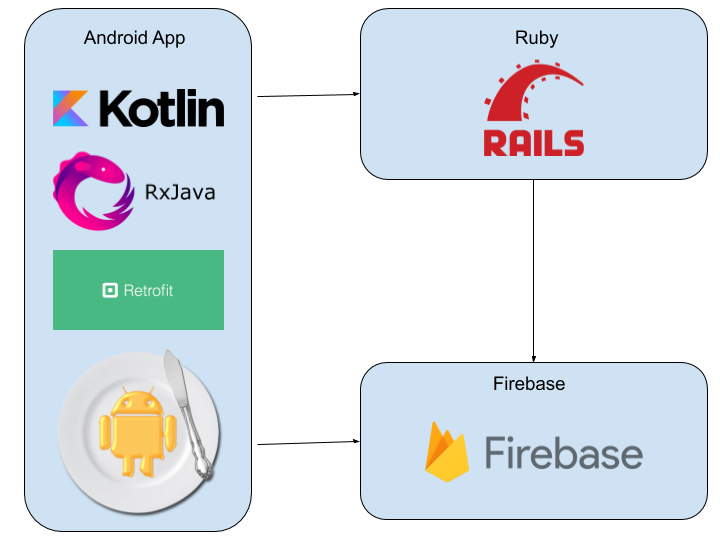
\includegraphics[width=0.7\textwidth]{SystemOverview.png}
  \caption[Overview of the Proposed System]{Overview of the Proposed System}
  \label{fig:systemoverview}
\end{figure}

As shown in Figure \ref{fig:systemoverview} the system consists of three parts, the Android mobile app, the Firebase backend and the Ruby backend.

The mobile app will communicate with both Firebase and the Ruby server as denoted by the arrows in the figure. The Ruby server will also have a communication to the Firebase backend in order to facilitate particular functionality such as notification scheduling as mentioned previously. 

It should be noted that the logos in Figure \ref{fig:systemoverview} represent the libraries used in each part of the system but this is not extensive, as some libraries simply do not have logos. A more complete list and their associated functionality is given in sections \ref{section:mobiletechused}, \ref{section:firebasetechused} and \ref{section:rubytechused}.

\subsection{Mobile App Technologies Used}
\label{section:mobiletechused}

\subsubsection{Language - Kotlin}
\label{arch:kotlin}

As outlined in section \ref{mobileapplicationsstateoftheart} Kotlin is now the language Google recommends for Android development. For this reason, and others outlined in section \ref{mobileapplicationsstateoftheart} Kotlin will be the language used for the Android app development aspect of this project rather than Java.

\subsubsection{Code Structure - Clean Architecture}
\label{section:cleanarch}

For the Android application aspect of this project the code will be using Clean Architecture, a code architecture developed by Robert Martin in his book "Clean Architecture: A Craftman's Guide to Software Structure and Design"\cite{cleanarchitecturebook}.

\begin{figure}[ht]
  \centering
      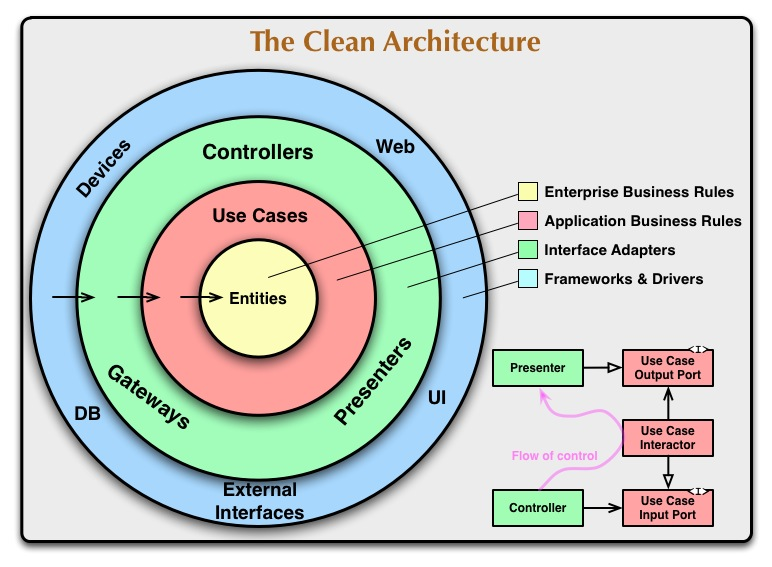
\includegraphics[width=0.7\textwidth]{cleanarchitecturemartinmodel.jpg}
  \caption[Clean Architecture Diagram]{Clean Architecture Diagram\cite{cleanarchitecturemartindiagram}}
  \label{fig:cleanarchitecturediagram}
\end{figure}

Figure \ref{fig:cleanarchitecturediagram} shows the approach to clean architecture as devised by Robert Martin. In this diagram the outer layers know about their immediate inner layer but holds no reference to any layer inside that. A layer also knows nothing of its outer layers.

This project will be using a slightly modified version of clean architecture which has been devised by the Android development team at the company Teamwork in order to handle some Android specific issues which this base version of clean architecture does not address.

\begin{figure}[ht]
  \centering
      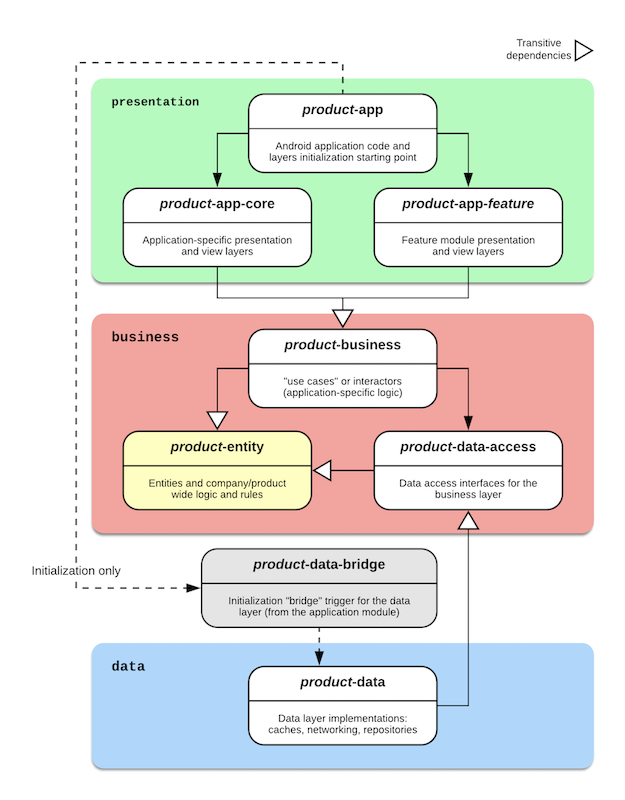
\includegraphics[width=0.7\textwidth]{clean_architecture_android_structure.png}
  \caption[Android Specific Clean Architecture Diagram]{Android Specific Clean Architecture Diagram\cite{teamworkcleanarchitecture}}
  \label{fig:teamworkcleanarchitecture}
\end{figure}

As seen in figure \ref{fig:teamworkcleanarchitecture} there are three distinct parts to this clean architecture setup, Data, Business and Presentation. In this implementation there are extra modules included to deal with Android specific problems in relation to clean architecture.

%The business-injection module is in place to allow the DI framework to successfully build a dependency graph in a multi-module project. 
The data-bridge modules exists only to initialise the DI graph for the data layer and contains no specific application logic.

The data layer covers operations related to network requests and database storage. In this project Firebase is used as the backend storage service and the Android libraries to access the Firebase API automatically handle caching. Therefore the data layer in this project will be used mainly for accessing Firebase but any extra work related to caching or threading will be unnecessary as the Firebase libraries handle these internally. The data layer will also be used to access the Ruby backend server but this will be in only limited circumstances given the relatively limited functionality of this server when compared to the Firebase backend.

The business layer is in charge of accessing the data layer functionality and applying any necessary application level business rules to the result obtained. This typically amounts to checking the validity of the data received and either just passing it on to the presentation layer when it is valid or passing some default value to the presentation layer when this data is not valid.

The presentation layer of this setup is in charge of calling the appropriate business layer methods when needed and obtaining a result. The presentation layer is also responsible for performing any transformations to the result obtained in order to make it suitable to show to the user.

While there are some clear cut differences between the presentation and business layers some functionality may seem like it could fall into either category. A common way of distinguishing responsibilities is to think of the presentation layer deciding the when and the business layer deciding the how. The presentation layer decides when something should be done, such as at the click of a button. The business layer decides how it should be done, for example whether it should happen asynchronously or not.

More in-depth detail on this exact clean architecture implementation can be found at \url{https://github.com/Teamwork/android-clean-architecture}. The only changes this project will make to this base setup is the conversion of any Java classes to Kotlin.

Clean Architecture will be employed extensively in this project as all classes in the mobile app will conform to  the layering and restrictions set on this layers by the Clean Architecture code structure.

\subsubsection{Dependency Injection - Dagger2}

This mobile app will use Dagger2 as the dependency injection framework of choice. While there are many DI frameworks available Dagger2 is maintained by Google and as seen in figure \ref{fig:androiddi} it is the only DI framework recommended for all sizes of Android app. 

\begin{figure}[ht]
  \centering
      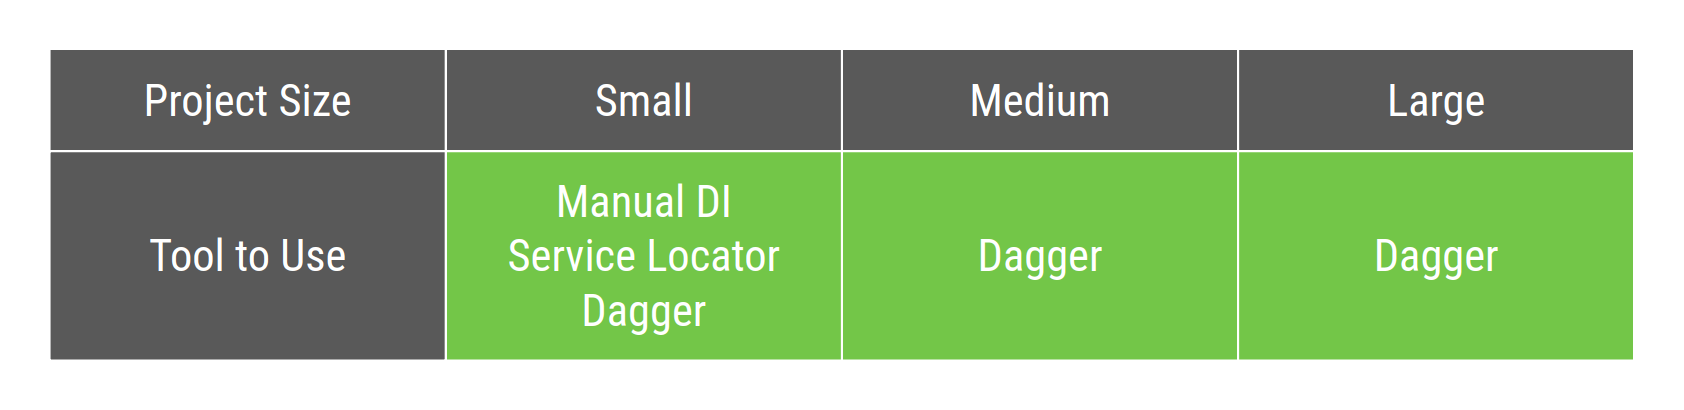
\includegraphics[width=0.7\textwidth]{androiddirecommendation.png}
  \caption[Android DI Framework Recommendations]{Android DI Framework Recommendations\cite{androiddi}}
  \label{fig:androiddi}
\end{figure}

The size of an Android app is based approximately on how many different screens it has. These approximate size definitions are outlined in figure \ref{fig:androidappsizes}.

\begin{figure}[ht]
  \centering
      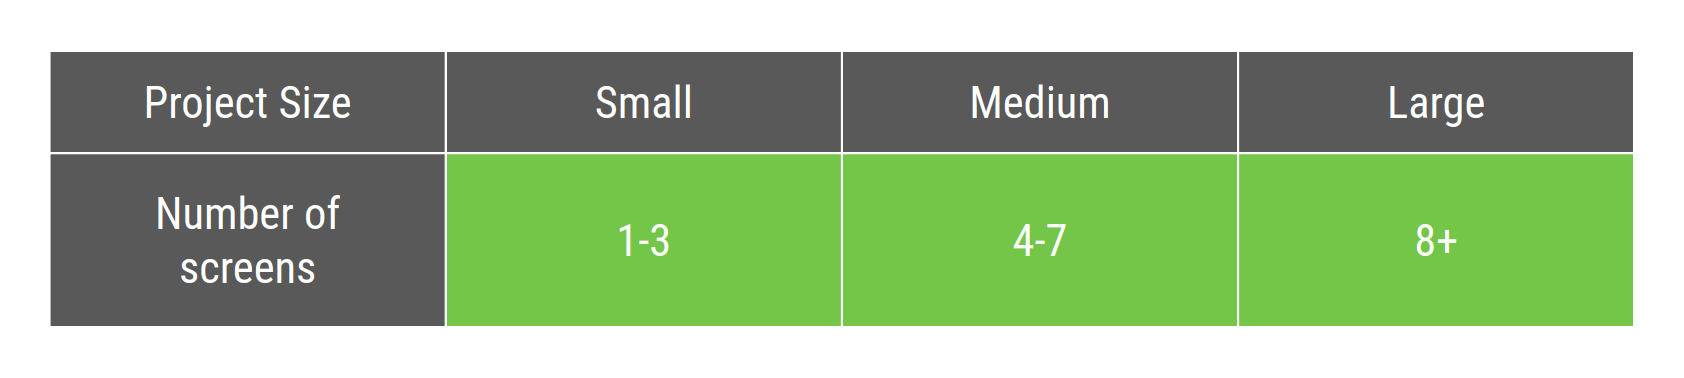
\includegraphics[width=0.7\textwidth]{appsizedef.png}
  \caption[Android App Size Approximations]{Android App Size Approximations\cite{androiddi}}
  \label{fig:androidappsizes}
\end{figure}

Dagger2 will be used extensively in this project as a means of keeping with the SOLID principles of Single Responsibility and Dependency Inversion. It is anticipated that almost all classes will use Dagger2 to inject dependencies.

\begin{figure}[ht]
  \centering
      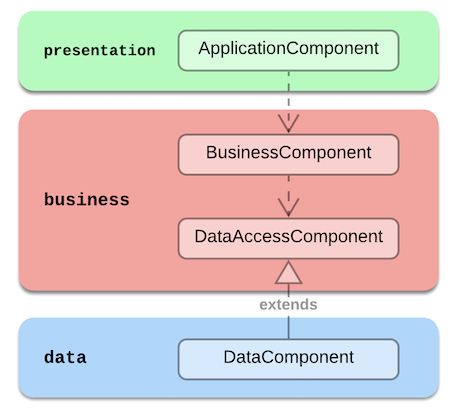
\includegraphics[width=0.7\textwidth]{clean_app_architecture_components.png}
  \caption[Dagger2 Component Graph Setup]{Dagger2 Component Graph Setup\cite{teamworkcleanarchitecture}}
  \label{fig:cleanarchitecturedicomponents}
\end{figure}

Shown in figure \ref{fig:cleanarchitecturedicomponents} is the setup for how Dagger2 will utilise multiple components in order to build a dependency graph across multiple modules

\subsubsection{AndroidX}

AndroidX refers to the Android support libraries which provide backwards compatibility to Android apps. It also encompasses Google's Android Jetpack suite of libraries.

AndroidX, despite officially being labelled as a group of support libraries, are a necessity in every Android project as many of the basic classes used in Android development come from it. There would therefore be far too much information to go into here if all AndroidX packages which are to be used were mentioned.

However, by leaving out the common uses of AndroidX which can be found in most, if not all, Android projects we can look at some of the more helpful features which come out of the Android Jetpack subset of libraries which will be used in this project.

\paragraph{Android KTX}

Android KTX acts as an add-on for the Kotlin language when used in Android. This library provides a set of extensions to Android classes which can replace verbose code with more concise versions which achieve the same functionality\cite{androidktx}.

\paragraph{Android Jetpack Navigation Component}

The Android Jetpack navigation component is a library which handles the boilerplate code associated with navigating between screens in an Android app.

While it makes up a minor part of mobile apps navigation in Android can often require a lot of boilerplate code to handle states. This code can often grow massive and lead it to be buggy and difficult to maintain.

The navigation component takes care of these problems as well as adding support for features which would normally be considered quite difficult to implement, such as deep linking.

In short the use of this library allows for a massive reduction in boilerplate code, handles difficult use cases and thus frees the developers time allowing them to focus on user facing features\cite{androidjetpacknavigation}.

There are many more helpful libraries available as part of the Android Jetpack suite. More information can be found on them at \url{https://developer.android.com/jetpack}.

The AndroidX libraries will be used heavily throughout this mobile app as they are now a standard in Android development and the exact uses are listed above.

\subsubsection{RxJava/RxAndroid}

RxJava is a library designed to allow for quick development of asynchronous and event-based programs using observable sequences\cite{rxjava}.

% This library uses an implementation of the Observer pattern to complete some background work then pass the result to a foreground thread.

By using RxJava and its RxAndroid extensions a lot of boilerplate code relating to threading can be avoided while also remaining conscious of the Android lifecycle with little effort on the part of the developer. 

% As RxJava is developed with asynchronous work in mind there is little for a developer to worry about in terms of race conditions or other common threading problems as these are handled by the library. 
\begin{figure}[ht]
  \centering
      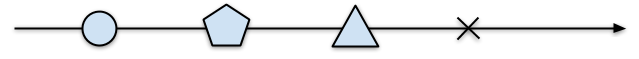
\includegraphics[width=0.7\textwidth]{rxjavabasicexample.png}
  \caption[RxJava Basic Observable Example]{RxJava Basic Observable Example\cite{rxjavamarblediagram}}
  \label{fig:rxjavamarblediagram}
\end{figure}

Figure \ref{fig:rxjavamarblediagram} shows one of the most basic examples of how RxJava emits items in an Observable. The arrow line indicates time passing. First the circle is emitted, then the pentagon, then the triangle and finally the thread terminates with an error. The thread can also continue on indefinitely or close without an error.

This is only one of the most basic examples with no other operations being performed on the items emitted. More detailed examples and diagrams can be found at \url{https://medium.com/@jshvarts/read-marble-diagrams-like-a-pro-3d72934d3ef5}.

The use of RxJava in this project will not be extensive as it is not anticipated for the use of separate threads to occur frequently. This is taking into account that Firebase, the main source of slow operations in this project, handles its own threads internally.

\subsubsection{Retrofit}

Retrofit is a library designed to turn a HTTP client into a Java interface. Retrofit essentially takes a remote REST API and by providing an interface which outlines the structure of the various request types the REST API uses, Retrofit handles generating the correct code for contacting the remote server with the query URL and all parameters formatted correctly\cite{retrofit}.

Retrofit will be playing a relatively small role in this project as it will only be used in interactions with the Ruby server which plays a limited role in this project.

Further information on Retrofit is used can be found at \url{https://square.github.io/retrofit/}.

\subsubsection{Butter Knife}

Butter Knife is a view binding library designed to reduce the boilerplate code associated with typical Android view binding by generating the necessary UI code at compile time\cite{butterknife}.

When a view exists but not in the same scope as the logic controller it is attached to, Android Studio will not recognise this mistake and allow a successful build despite the fact it won't work. By using Butter Knife an error is thrown at compile time which highlights this issue.

Butter Knife will be used quite extensively in this project as it will be in use in every screen presented to the user to bind all UI elements.

Further details on Butter Knife can be found at \url{https://jakewharton.github.io/butterknife/}.

\subsubsection{Glide}

Glide is an image loading and caching library for Android which handles all loading asynchronously. By using this library there is a massive reduction in boilerplate code and the developer can avoid working with difficult issues in regard to threading and background operations, as well as massively improving efficiency on the time-consuming and resource heavy task of image loading in Android.

Glide will not be used very much in this project as it is anticipated to be used mainly when loading images which are stored online, such as user profile pictures. All other images will be either packaged with the app or defined as vector images using XML.

Further details on the usage of Glide can be found at \url{https://github.com/bumptech/glide/blob/master/README.md}.

\subsubsection{Moshi}

Moshi is a library for converting JSON responses to POJO and vice versa.\cite{moshi}. It holds some significant improvements over similar libraries such as GSON in regards to speed and Kotlin support\cite{moshibettergson}.

Moshi will play a relatively small part in this project as it will be used only for interactions with the Ruby backend server and, as stated previously, this server will have a limited role in comparison to the Firebase backend.

\subsection{Firebase Technologies Used}
\label{section:firebasetechused}

\begin{figure}[ht]
  \centering
      
\includegraphics[width=0.7\textwidth]{Firebase_Logo.png}
  \caption[Firebase Logo]{Firebase Logo\cite{firebaselogo}}
  \label{fig:firebaselogo}
\end{figure}

While Firebase is technically a single technology provider, it encompasses many different types of features so it is still worth outlining here which of these will be used in this project.

\subsubsection{Firebase Authentication}

Firebase Authentication provides a drop-in UI solution for including a complete register and login flow in a mobile app. There are a lot of built in options such as allowing sign-in through Twitter, Google and other sites but for this project the default email and password sign-in will be used.

A detailed overview of Firebase Authentication can be found at \url{https://firebase.google.com/docs/auth}.

Firebase Authentication will form the one and only register and login procedure for users in this project. The Firebase UI for registering or logging in will be the first screen presented to the user on startup of the app. Once signed in, it is expected that this screen will rarely, if ever, be used again by the user. As with most services requiring authentication it is expected that once signed in a user will not sign out again for the sake of convenience.

\subsubsection{Firebase Cloud Firestore}

Firebase Cloud Firestore is a realtime NoSQL cloud based storage solution which allows for many clients to quickly access up-to-date information.

\begin{figure}[ht]
  \centering
      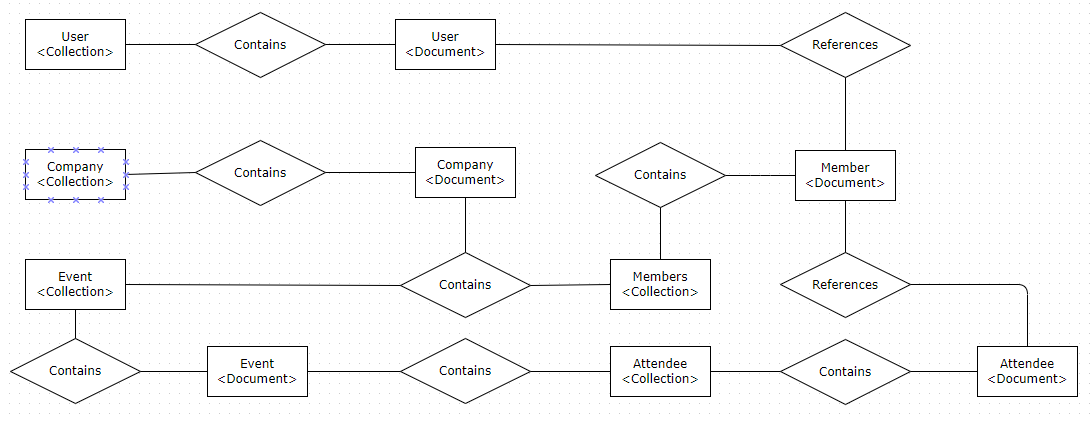
\includegraphics[width=0.7\textwidth]{DBDesign.PNG}
  \caption[Proposed Database Design]{Proposed Database Design}
  \label{fig:databasedesign}
\end{figure}

In Figure \ref{fig:databasedesign} is the proposed design of the Firestore NoSQL database. 

The structure of the Firestore database is a document-based NoSQL database, each document is made up of key-value pairs for the data and subcollections which contain further collections of documents. 

In this diagram we can see collections contain documents and documents, in turn, may contain collections. Unfortunately, due to the lack of a strictly enforced data structure as with SQL databases, many modelling tools for NoSQL databases do not seem to contain the tools for detailing key-value pairs of data.

The two main collections making up this database will be 'User' and 'Company'. These then contain documents of an individual User or Company in turn. While the User collection remains simplistic, the Company collection is more complicated due to the data points associated with a company in this project. 

Each Company document will contain the subcollections of 'Event' and 'Members'. Each Member document will reference an already existing User document. Each Event document will contain a further subcollection of 'Attendees' with each Attendee document referencing a company member.

Aside from any subcollections each document will also contain any other required information for its data. For example an Event document will contain event name, location and so forth on top of its Attendees subcollection. 

The exact features of Firestore are far too extensive to list here but details can be viewed at \url{https://firebase.google.com/docs/database/rtdb-vs-firestore}.

Firestore will be used extensively in almost every facet of this project as it will need to be accessed by the mobile app for every display of information as well as by the Ruby server to allow for the required database access.

\subsubsection{Firebase Cloud Messaging}

FCM is a component of Firebase which allows for sending messages reliably to connected client devices. In the case of mobile devices, these are almost always then shown as notifications.

Further details on FCM can be found at \url{https://firebase.google.com/docs/cloud-messaging}.

FCM will be used for all instances of notification delivery in this project.

\subsection{Ruby Server Technologies Used}
\label{section:rubytechused}

\subsubsection{Ruby on Rails}

\begin{figure}[ht]
  \centering
      
\includegraphics[width=0.7\textwidth]{railslogo2.png}
  \caption[Ruby on Rails Logo]{Ruby on Rails Logo\cite{rubyonrailslogo}}
  \label{fig:rubyonrailslogo}
\end{figure}

Ruby on Rails is a library for the Ruby language which provides an easy to setup environment and quick development of applications\cite{rubyonrails}.

As this project will be using the Ruby server in a limited number of cases and purely as an API, Ruby on Rails is chosen as it provides built-in tools for creating exactly this kind of setup quickly\cite{rubyonrailsapi}.

Rails applications also come with a default database using SQLite. In this project the data storage will be handled primarily by Firebase, however as the ruby server is required to generate a human readable ID for each new company created, this SQLite database will be used as a convenient way to auto-generate an ID for new companies. This will then be stored by Firebase with all other data\cite{rubydatabase}.

Rails also gives the benefit of strictly enforcing an MVC code architecture which in turn tends to produce more robust code\cite{rubycodestructure}.

Further details on Ruby on Rails can be found at \url{https://rubyonrails.org/}. Details on specifically the API features of Rails can be found at \url{https://guides.rubyonrails.org/api_app.html}.

Rails will form the entirety of the Ruby server in this project.

\subsection{How These Technologies Are Used}

The proposed use of the outlined technologies and the interactions between different parts of the system are as follows:

The mobile app code structure will be using Clean Architecture as detailed in section \ref{section:cleanarch}. In an effort to make code as reusable as possible and to increase adherence to the SOLID principles of Single Responsibility and Dependency Inversion, Dagger2 will be used to provide instances of all possible classes throughout the project.

The mobile app will need to have means of communication with both Firebase and the Ruby server. Firebase includes all networking and threading operations as part of its libraries but connection with the Ruby server will need to be handled by the developer. In this scenario RxJava, Retrofit and Moshi are all used. Retrofit is the means of connecting to the server and receiving a response, Moshi will parse that response into usable objects in code and RxJava will handle the threading operations which come with networking functionality.

As listed in section \ref{section:mobiletechused} other libraries such as Glide and the AndroidX suite will be used. The AndroidX libraries will be used extensively for various pieces of functionality throughout the app. Glide will be used in far more limited cases. In order to avoid too much repetition here on what functionality these libraries offer details can be found above in section \ref{section:mobiletechused} giving an overview of their benefits.

The Firebase backend will provide most of the server side functionality for this project, most heavily used will be Firebase Cloud Firestore for storing user data.

The separate Firebase components listed in section \ref{section:firebasetechused} will not actually have any direct interaction with one another in this project.

Most interactions with the Firebase backend will come from the mobile app through the use of the various Firebase libraries. Firebase Cloud Storage will be in charge of providing the data on events, people and companies. Firebase authentication will provide the means of new users registering and logging into the mobile app and FCM will provide the mechanism for sending notifications to users at the appropriate times, such as for event invitations, reminders and so forth.

Finally the Ruby server will provide some limited functionality which Firebase does not support currently. Within the scope of this part of the system is creating a new company ID and scheduling when notifications are to be sent.

The Ruby server is in charge of creating a new company ID as it provides a convenient way of generating unique human readable IDs for each company whereas Firebase Cloud Storage does not. By default Ruby on Rails comes will an SQLite database. This database will not be used for data storage but by creating a new entry for each new company the auto-generated ID created by the database gives a simple unique value which can then be passed onto Firebase.

Firebase does not currently support sending a notification at a specific time but by including the Ruby server in the notification process a workaround can be found. When some action is taken which results in notifications being sent sometime in the future the Ruby server can schedule when to connect to Firebase and send the notification.

For these purposes there will also e a direct means of interaction between the Ruby server and the Firebase backend.

\section{Risk Assessment}
\label{section:risks}
% Identify any potential risk precluding you from successfully complete your project. This section is really important and often neglected by students resulting in fatal risks occurring in some projects. Make sure to give this section the time it requires. Classify the risk according to their importance, possibility of arising and enumerate the decisions you can make to anticipate them or mitigate them (in case they finally arise). Table \ref{tab:ProjRisks} may help with this classification. This section should include your mitigation approach for any critical risks.

% \begin{table}[h]
% \centering
% \scriptsize
% \caption{Initial risk matrix}
% \begin{tabular}{|p{2cm}|p{2cm}|p{2cm}| p{2cm} |p{2cm}| p{2cm}|}
% \hline \bf Frequency/ Consequence & \bf 1-Rare & \bf 2-Remote & \bf 3-Occasional & \bf 4-Probable & \bf 5-Frequent\\ [10pt]

% \hline \bf 4-Fatal & \cellcolor{yellow!50} & \cellcolor{red!50} & \cellcolor{red!50} & \cellcolor{red!50} &\cellcolor{red!50} \\ [10pt]

% \hline \bf 3-Critical &\cellcolor{green!50} & \cellcolor{yellow!50} & \cellcolor{yellow!50} & \cellcolor{red!50} &\cellcolor{red!50} \\ [10pt]

% \hline \bf 2-Major & \cellcolor{green!50} & \cellcolor{green!50} & \cellcolor{yellow!50} &\cellcolor{yellow!50} &\cellcolor{red!50} \\ [10pt]

% \hline \bf 1-Minor & \cellcolor{green!50} & \cellcolor{green!50} & \cellcolor{green!50} &\cellcolor{yellow!50} &\cellcolor{yellow!50} \\ [10pt]
% \hline
% \end{tabular} \\
% \label{tab:ProjRisks}
% \end{table}

\subsection{Risk No. 1}

\textbf{Description}

Firebase backend goes down.

\textbf{Consequences}

Newly entered information from Firestore will not be made available to users.

\textbf{Severity}

Critical

\textbf{Possibility of Occurring}

Rare

\textbf{Risk Mitigations}

Unfortunately not much can be done in the event that Firestore somehow becomes unresponsive as this is the backbone of the app. However as Firebase is owned and backed by Google the odds of the service becoming unresponsive are incredibly rare. 

Besides this the Firestore library for Android comes with caching functionality built in. In such an event users will still be able to view the latest cached information on their device, also any newly entered data will be cached until such time as it can be persisted to the cloud based backend.

\subsection{Risk No. 2}

\textbf{Description}

Unable to complete sprints due to time constraints

\textbf{Consequences}

In such a case the app will be missing planned features and bugs may not be fixed.

\textbf{Severity}

Major

\textbf{Probability of Occurring}

Probable

\textbf{Risk Mitigations}

The chances of this occurring in the development of the Ruby backend or the Firebase setup is very unlikely given the limited functionality and ease of setup of these two parts of this project. This risk is therefore almost entirely a risk for the mobile app development.

The only mitigation in this scenario is to consistently follow the sprint outline devised in section \ref{section:implementationplan} and, when possible, get to work on the next sprint early.

By doing this and strictly following the concept of the MVP of this app, the project development phase can still end with an app which provides a high degree of value despite missing some planned features/functionality.

\subsection{Risk No. 3}

\textbf{Description}

Functionality differences between Android OS versions

\textbf{Consequences}

Users on different Android OS versions, particularly older versions, may experience non-typical or unexpected behaviour when using the app.

\textbf{Severity}

Minor

\textbf{Possibility of Occurring}

Probable

\textbf{Risk Mitigations}

While this is an issue known to occur in Android apps it is incredibly rare that this the actual logic of the app. What is far more common is that UI elements are affected by this issue in that styling may not be applied correctly and thus UI elements which employ certain known troublesome classes can appear differently depending on OS version.

While this risk is probable in its likelihood to happen, the chances of it adversely affecting  a user and preventing them from using the app is practically non-existent. 

These issues most commonly occur on devices running Android OS version 22 or lower. Therefore to mitigate this issue, and to allow reduction in handling various edge cases which come with older Android versions, this project will set Android version 23 as the minimum OS version the app can be used on.

Furthermore there are also well known workarounds for these styling issues which should be employed consistently over the standard classes provided for styling which in turn will yield consistent results across devices.

\section{Methodology}
\label{section:methodology}
% Describe your personal approach on how to tackle the different parts of this project, including:
% \begin{itemize}
%     \item How to tackle the needed research to fulfill the background chapter. 
%     \item How to set up your Computer Science skills to the project needs (e.g., describe your plan to learn any new technology involved on the project that you are not familiar with). 
%     \item What core project managing approach will you follow (e.g., Waterfall, Scrum, etc).
% \end{itemize}

\subsection{Learning New Technologies}

In regard to learning new technologies I am already somewhat well experienced in working with Android including each of the libraries listed in section \ref{section:mobiletechused}. I have also used each of the Firebase features listed in section \ref{section:firebasetechused} quite extensively in the past.

The main part of this project implementation requiring practice and research is the use of Ruby on Rails for the server backend. Due to the relatively limited scope of the Ruby server and the expected time constraints by the time the implementation phase of this project comes about, the plan for learning how to use this technology will focus only on learning what is absolutely needed rather than obtaining a broad knowledge. 

I have already taken steps in reviewing how to setup a Ruby on Rails server which acts only as an API interface. 

From this initial learning I believe the Ruby aspect of this project will be relatively short as Rails provides a quick setup tool for this exact use case. Further to this the Firebase documentation provides various examples of using Firebase in Ruby. Given these factors the Ruby part of this project is expected to be short and, relative to everything else, quite simple.

\subsection{Project Management Approach}

The development approach to be taken in this project will be Scrum with a sprint time of 2 weeks.

\section{Implementation Plan Schedule}
\label{section:implementationplan}
% Come up with a schedule for the remaining time (including second semester), so as to describe how do you envision to achieve the implementation of your project by the end of semester 2. This plan SHOULD be ambitious but MUST be realistic and SHOULD be informed by early prototyping and MUST be discussed with your term 1 supervisor.

\begin{longtable}{ |p{4cm}|p{10cm}|  }
		\hline
		\hline
		\textbf{Starting Date} & \textbf{Working On} \\
		\hline
		January 6th & 
		\begin{itemize}
		    \item Setup FirebaseAuth
		    \item Setup Firebase Cloud Storage
		    \item Setup FCM
		    \item Setup clean architecture mobile project structure
		    \item Setup Ruby on Rails for Ruby backend
		\end{itemize}\\
		\hline
		January 20th & 
		\begin{itemize}
		    \item Add FirebaseAuth to mobile app to allow for sign up/sign in
		    \item Create Ruby API for adding a new company
		    \item Add new company to Firebase Cloud Storage from Ruby server
		    \item Create mobile frontend for adding a new company
		    \item Create mobile frontend for users to join a new company
		    \item Create mobile frontend for users to view the events they are invited to
		\end{itemize}\\
		\hline
		February 3rd & 
		\begin{itemize}
		    \item Create mobile frontend for an admin to create a new event
		    \item An admin can set event-specific user details
		    \item Allow users to view the list of members of their company
		\end{itemize}\\
		\hline
		February 17th & 
		\begin{itemize}
		    \item Allow users to respond to an event invite
		    \item A user will receive a notification when invited to an event
		    \item A user can respond to event invites directly from the notification
		    \item A user will receive a notification for an upcoming event
		\end{itemize}\\
		\hline
		March 2nd & 
		\begin{itemize}
		    \item Update event details screen to show event location on a map
		    \item Implement app rating to allow users to give feedback on ease of use and reduction in difficulties experienced
		    \item Add mobile frontend to allow a user to view their own profile
		    \item Allow a user to view another user's profile
		\end{itemize}\\
		\hline
		March 16th &
		\begin{itemize}
		    \item Create mobile frontend for admins to view membership requests
		    \item Update join company functionality to now make a request rather than immediately join
		    \item Allow a user can edit their own profile
		\end{itemize}\\
		\hline
		April 6th &
		\begin{itemize}
		    \item An admin can set times for event reminders
		    \item An admin can make another user an admin
		\end{itemize}\\
		\hline
    \caption{Sprint Schedule}
	\label{table:sprints}
\end{longtable}

The remainder of the project implementation phase will be dedicated to working on any bug fixes or improvements which should be made to the system. The remaining time is also partially set aside for working on the implementation report.

\section{Evaluation}
\label{section:evaluation}
% Come up with an evaluation plan that allows you to measure how much have you actually achieved the goals of your project. This again is a section that is often neglected where students loose marks. How do you plan to measure the output of your project? A binary it works/does not work is insufficient. You need to be able to quantify the success against both the functional requirements and the initial idea. These are not the same as you may meet all function requirements outlined but not solve the overall problem because you have failed to revisit these and update them with new information which you learn as you are developing the project.

As shown in section \ref{section:implementationplan}, in the sprint beginning February 17th, one of the goals for this sprint is to implement user feedback.

This will be the way in which users can give a rating on the app, the usual 1 - 5 stars, as well as include any comments they have to give. As this app is the only user facing portion of the project any issues which occur due to problems in the Ruby or Firebase backends will also be reflected in this rating.

The top apps on the Google Play Store tend to have a rating of roughly 4 stars\cite{appstorerating}. Quite often 4 stars tends to be the minimum rating which apps aim to achieve therefore the same idea will be applied here. by taking the in-app star rating as a percentage, a score of 80\% or more will be taken to mean the project has been successful in achieving its goals.

Despite referencing Google Play Store ratings here the proposed user feedback will be separate. It will follow a very similar concept but by making this an in-app rating, customisations can be made on the type of feedback given. Feedback can be requested on very specific metrics, such as ease of event creation, reduction in organisation difficulties compared to previously used event management systems and so forth. This kind of feedback would prove far more useful than the generic good or bad review which is typically left on the Play Store. This feedback can then also be aggregated in Firebase to more easily allow for any desired data analysis.

\section{Prototype}
\label{section:prototype}
% Although you do not have a fully functional project yet, you should show wireframes, snapshots or representation on how do you envision your project to look once the implementation phase has been completed. The nature of this section will vary significantly from project to project and can include anything from code snippets to snapshots of service deployments. Any prototyping you have done during the term should be summarized here that has not been captured in earlier sections. For example if you are planning to host your project using AWS in an EC2 instance you should have at least created a "hello world" setup to determine the basics, this probably should have been discussed in section \ref{sec:Arch}.

This section gives a general idea on the look and functionality of the finished project. A prototype for the Firebase implementation is not included in this section as Firebase is a third party backend implementation which requires a client to work. Therefore the results of data stored by Firebase or notifications sent are shown as part of the mobile app prototype. 

All features in the mobile app prototype are shown but some of these will be unavailable if the user is not an admin. These will be highlighted in section \ref{section:mobileappprototype} when appropriate.

\subsection{Mobile App Prototype}
\label{section:mobileappprototype}

\begin{figure}[ht]
  \centering
      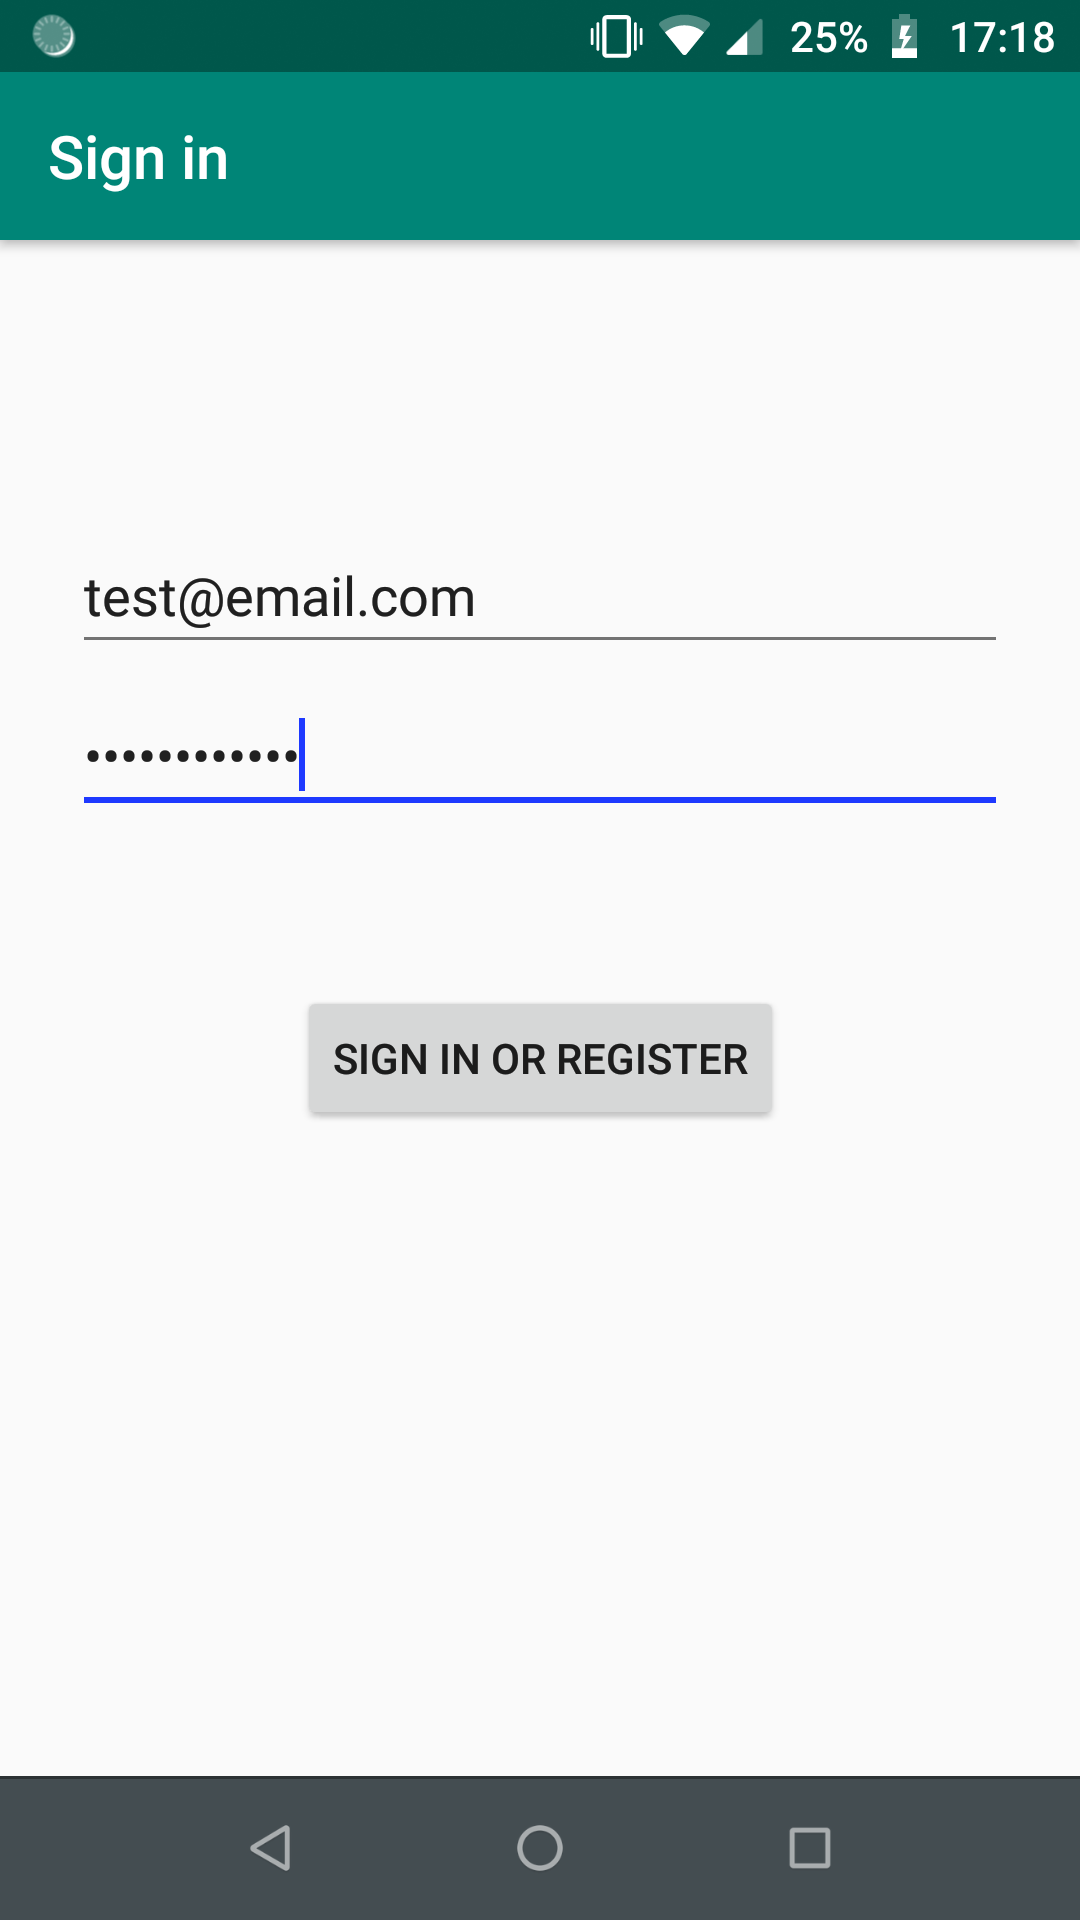
\includegraphics[width=0.7\textwidth]{SignInRegister.png}
  \caption[Mobile App Prototype Sign In/Register Screen]{Mobile App Prototype Sign In/Register Screen}
  \label{fig:signInRegister}
\end{figure}

Shown in Figure \ref{fig:signInRegister} is the outline of the Sign In/ Register screen for users to create an account for themselves or sign into an existing account. In the final project this screen will be handled by Firebase Authentication which provides a built-in sign in and register UI.

\clearpage
\begin{figure}[ht]
  \centering
      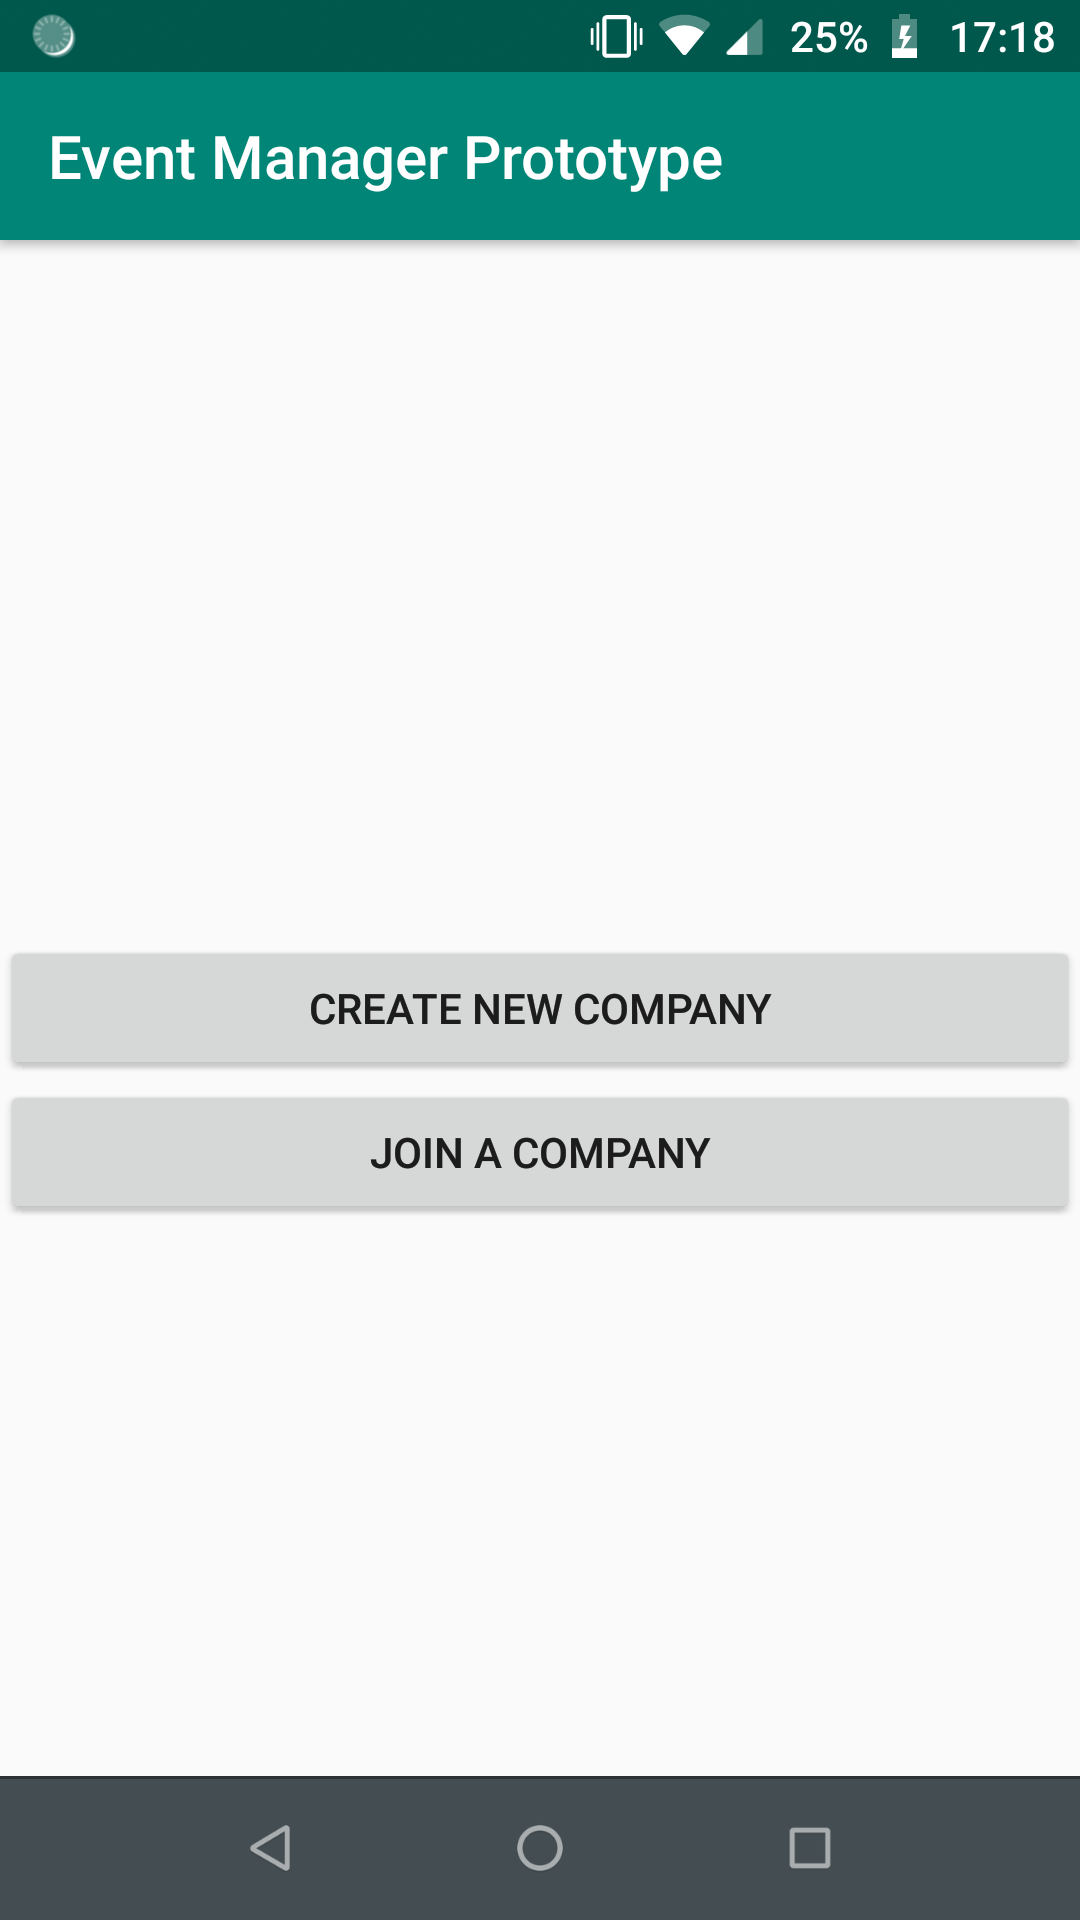
\includegraphics[width=0.7\textwidth]{CreateJoinCompany.png}
  \caption[Mobile App Prototype Create/Join Company Screen]{Mobile App Prototype Create/Join Company Screen}
  \label{fig:CreateJoinCompany}
\end{figure}

Once a user has created their account they will presented with the screen shown in Figure \ref{fig:CreateJoinCompany}. Here they will be presented with the option of either creating a new company or joining an already existing company.

\clearpage
\begin{figure}
\centering     %%% not \center
\subfigure[Create Company Screen]{\label{fig:a}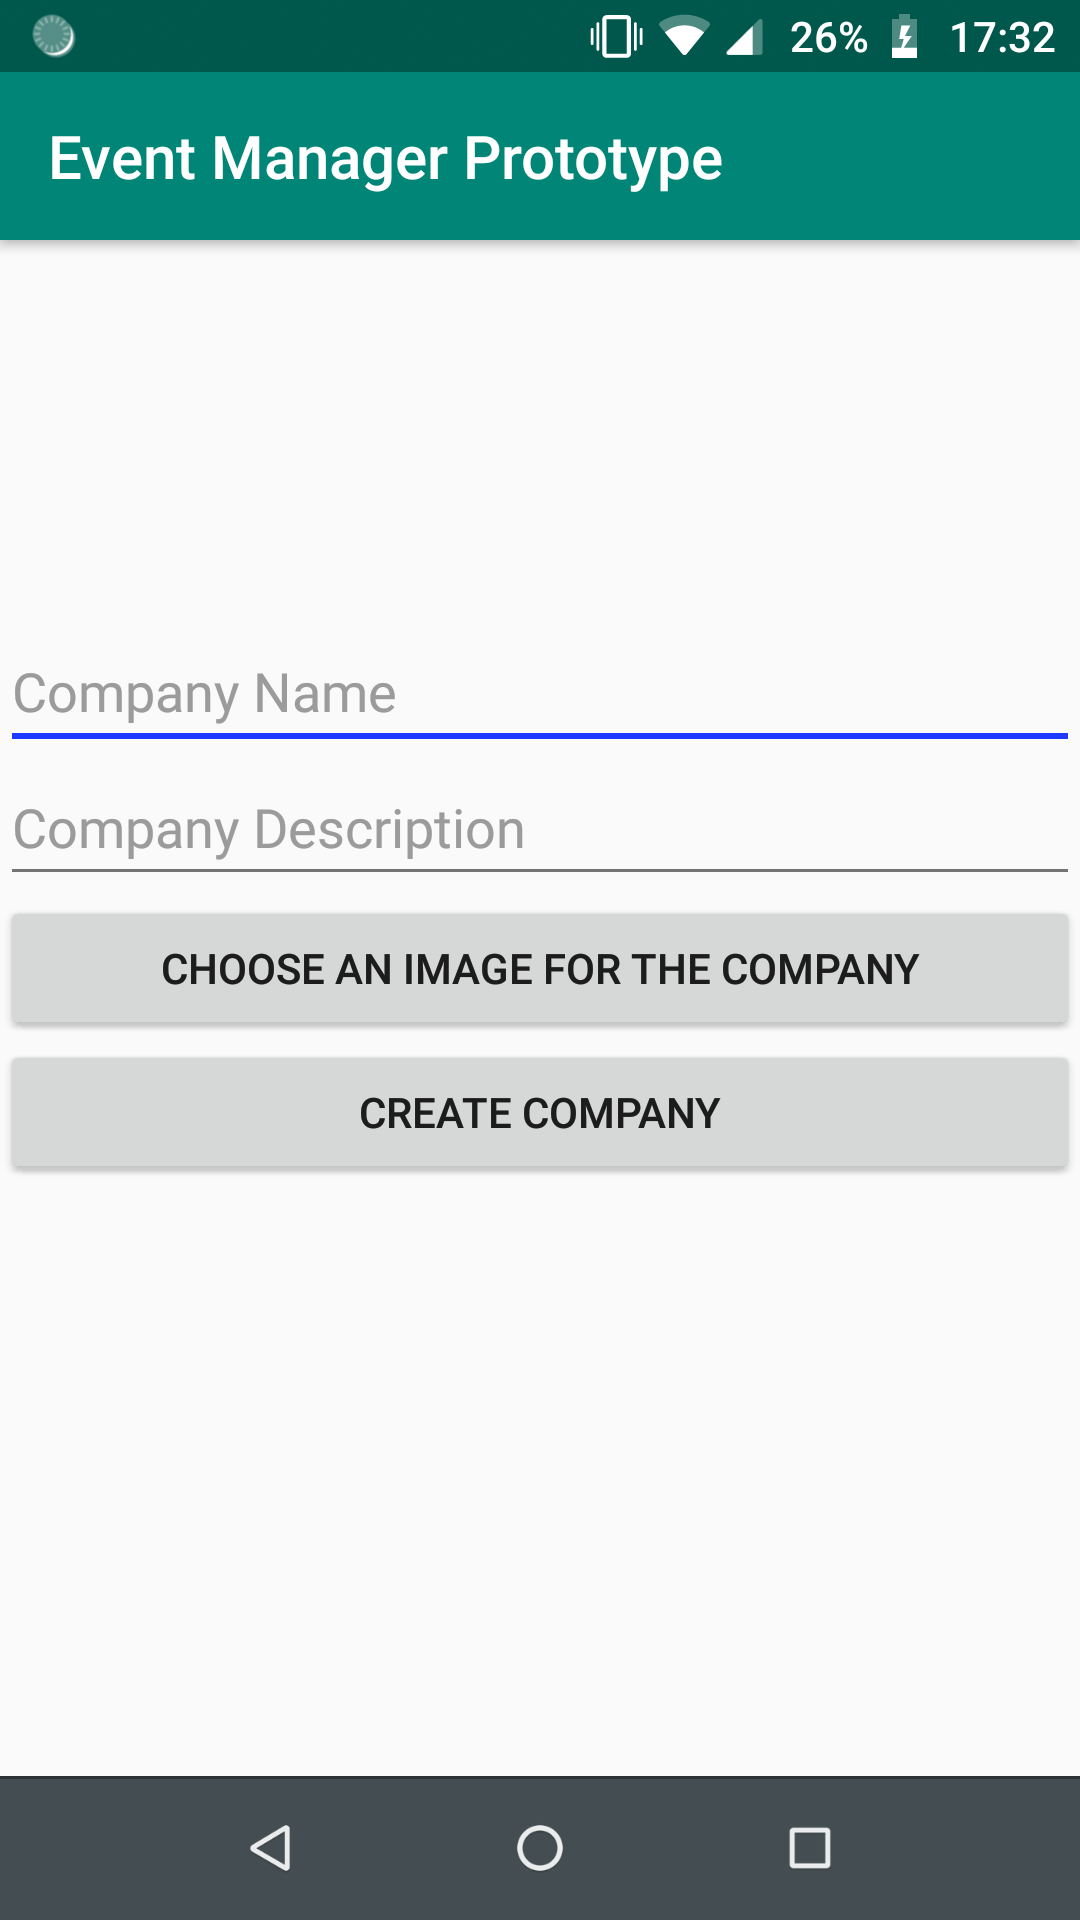
\includegraphics[width=0.48\textwidth]{CreateCompany.png}}
\subfigure[Join Company Screen]{\label{fig:b}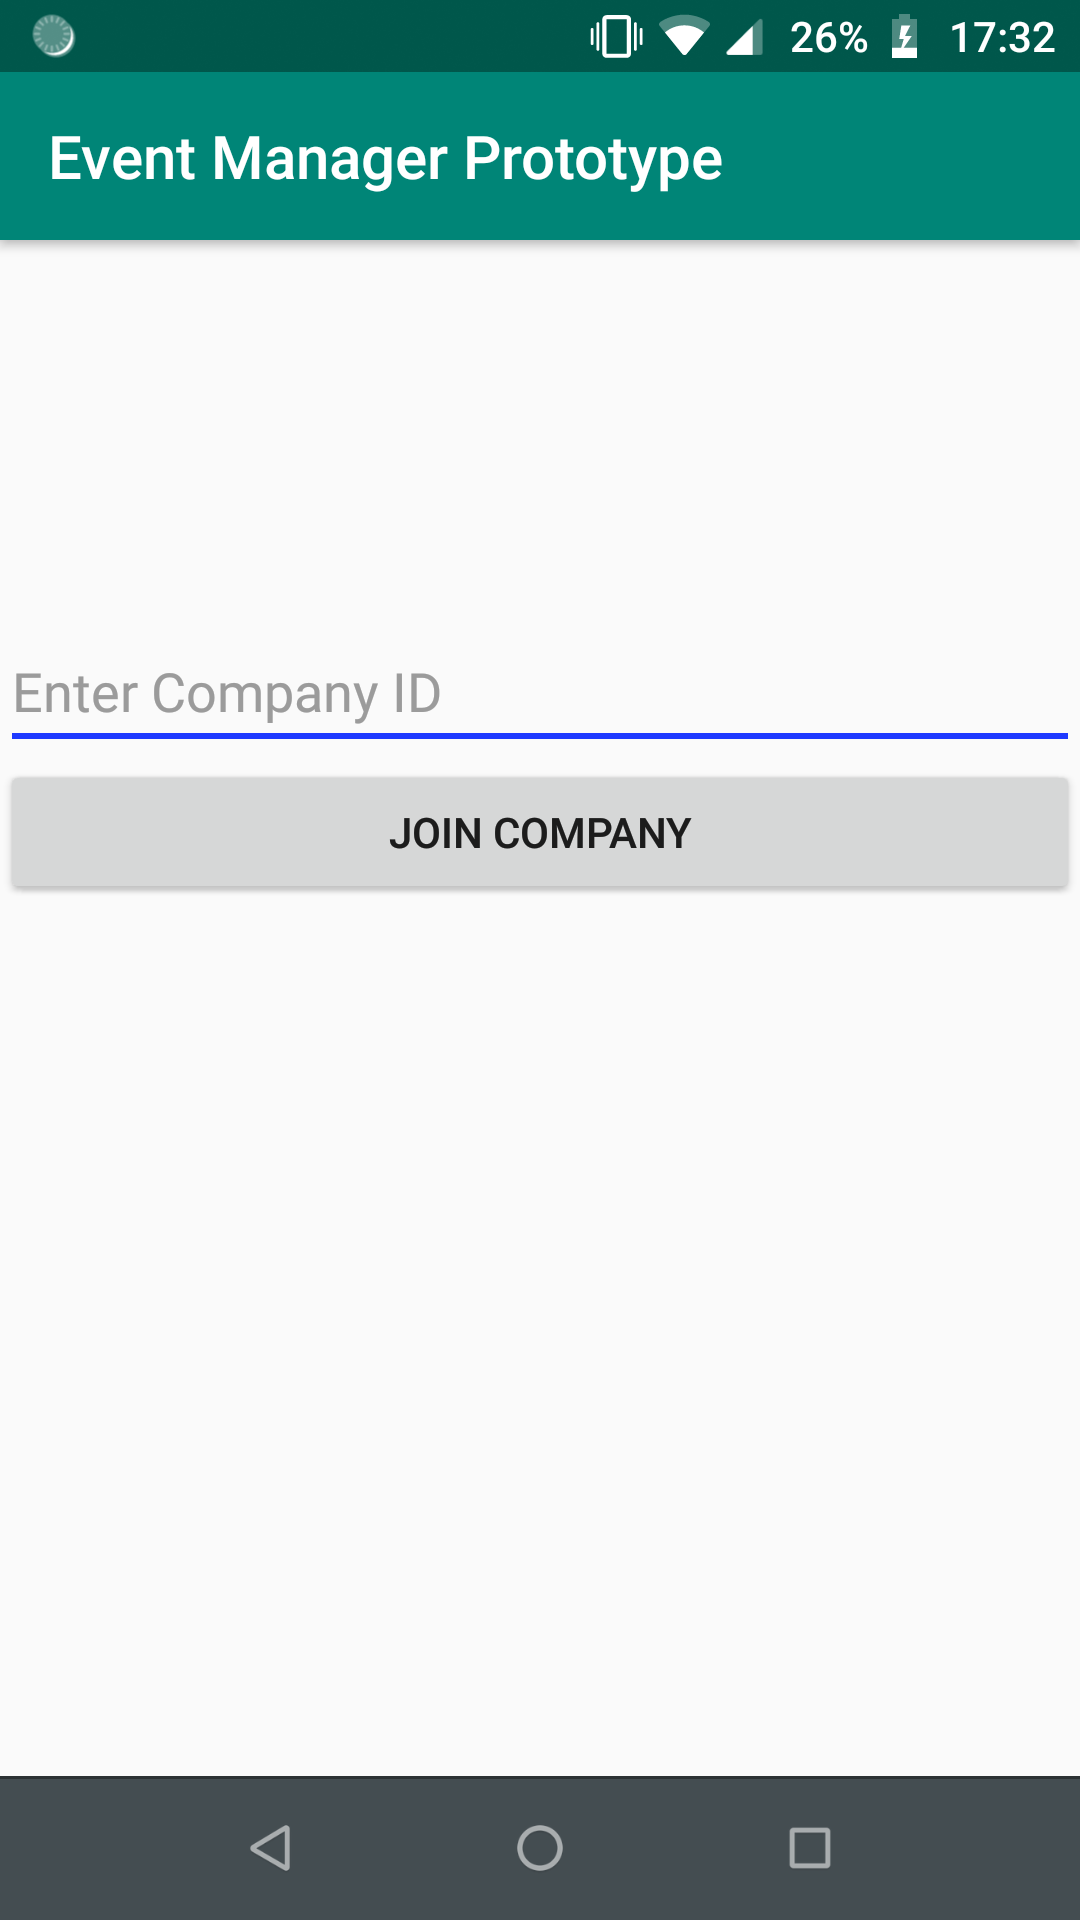
\includegraphics[width=0.48\textwidth]{JoinCompany.png}}
\caption{Mobile App Prototype Create and Join Company Screens}
\label{fig:CreateAndJoinCompanyScreens}
\end{figure}

Following on from the options presented in Figure \ref{fig:CreateJoinCompany}, in Figure \ref{fig:CreateAndJoinCompanyScreens} is shown the new options presented depending whether a user has chosen to create a new company of join an existing one. 

For creating a company the user can enter the company name, a description of the company and choose a company image. When joining a company a user must simply enter the company ID to make a membership request.

\clearpage
\begin{figure}[ht]
  \centering
      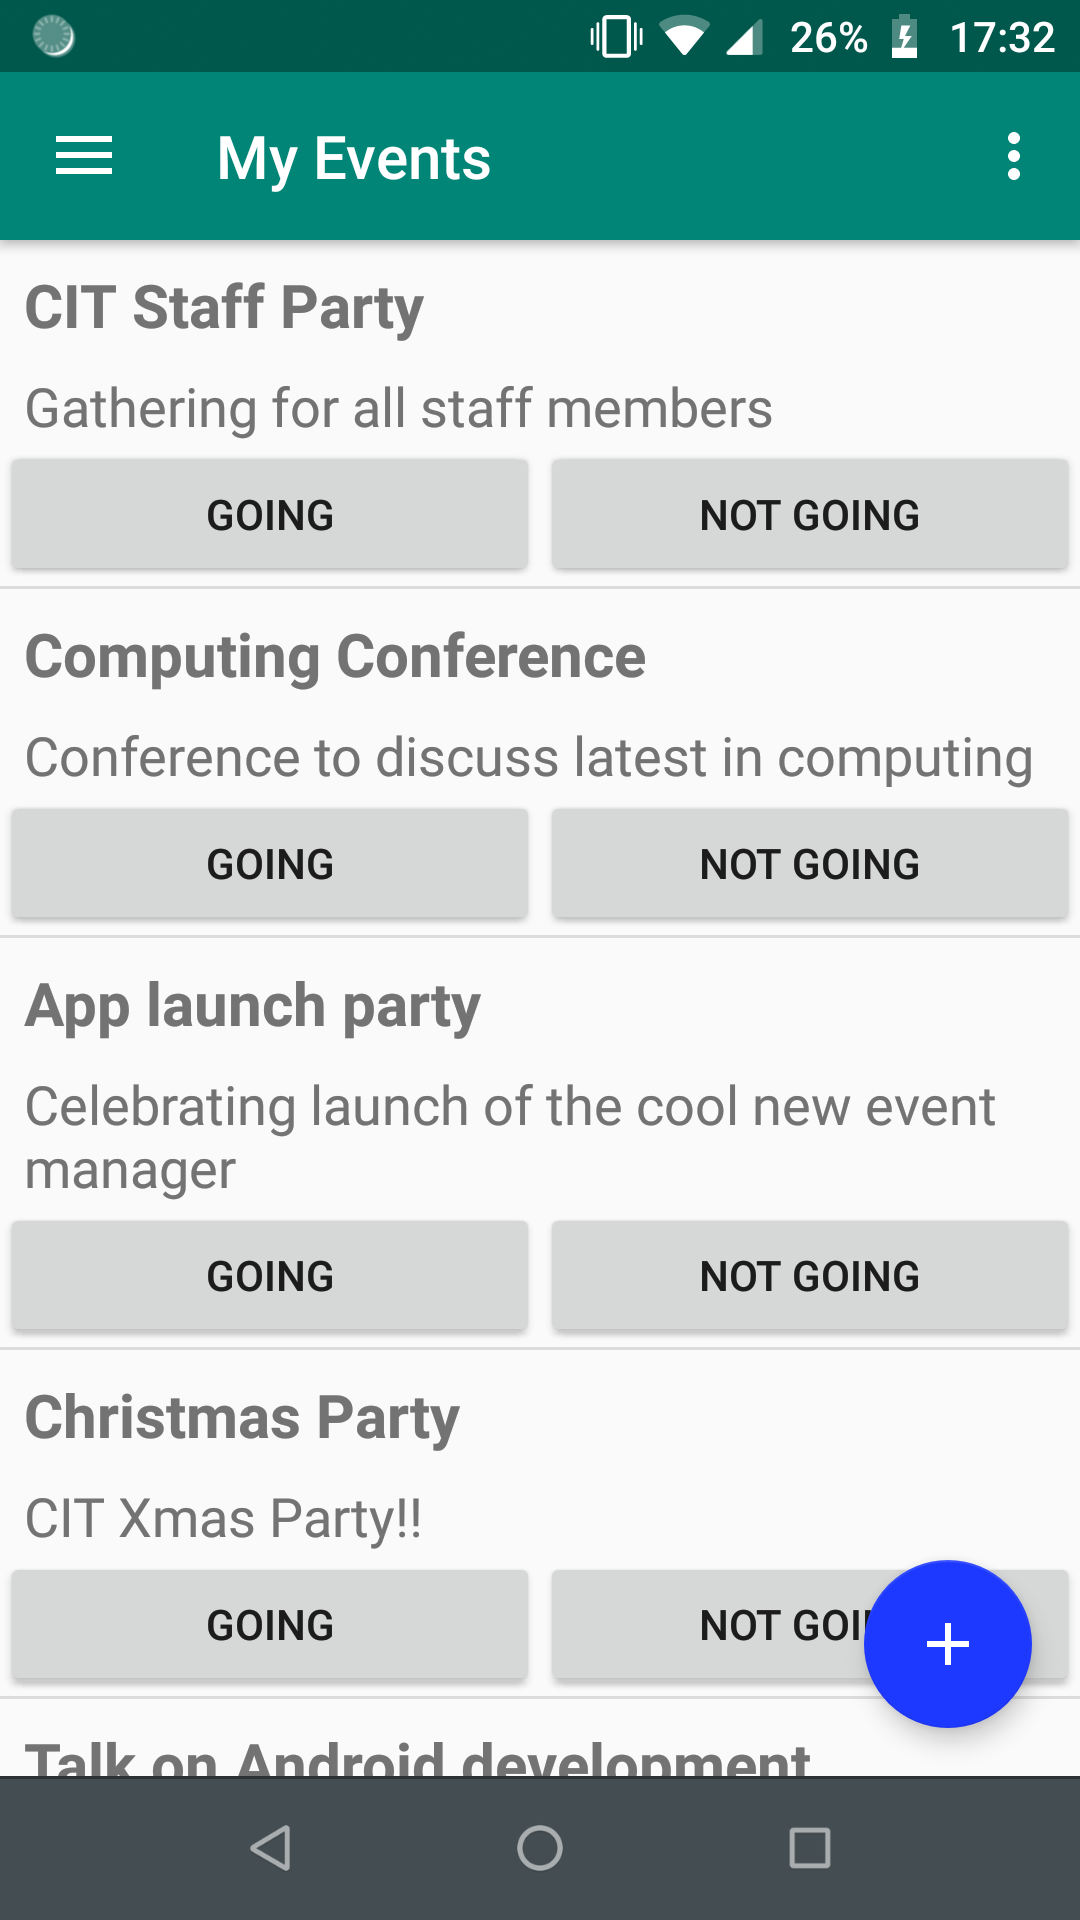
\includegraphics[width=0.7\textwidth]{EventList.png}
  \caption[Mobile App Prototype Event List]{Mobile App Prototype Event List}
  \label{fig:EventList}
\end{figure}

After completing the sign in and company creation process a user is able to gain full access to the app's features. First to be shown is the list of events as shown in Figure \ref{fig:EventList}. This screen shows the list of events the user is invited to and provides options for responding to those invites.

Also provided in this screen is a means of creating a new event through the blue '+' button in the lower right hand corner. This is a feature available to admins only. For users who are not admins this button will not be shown.

\begin{figure}[ht]
  \centering
      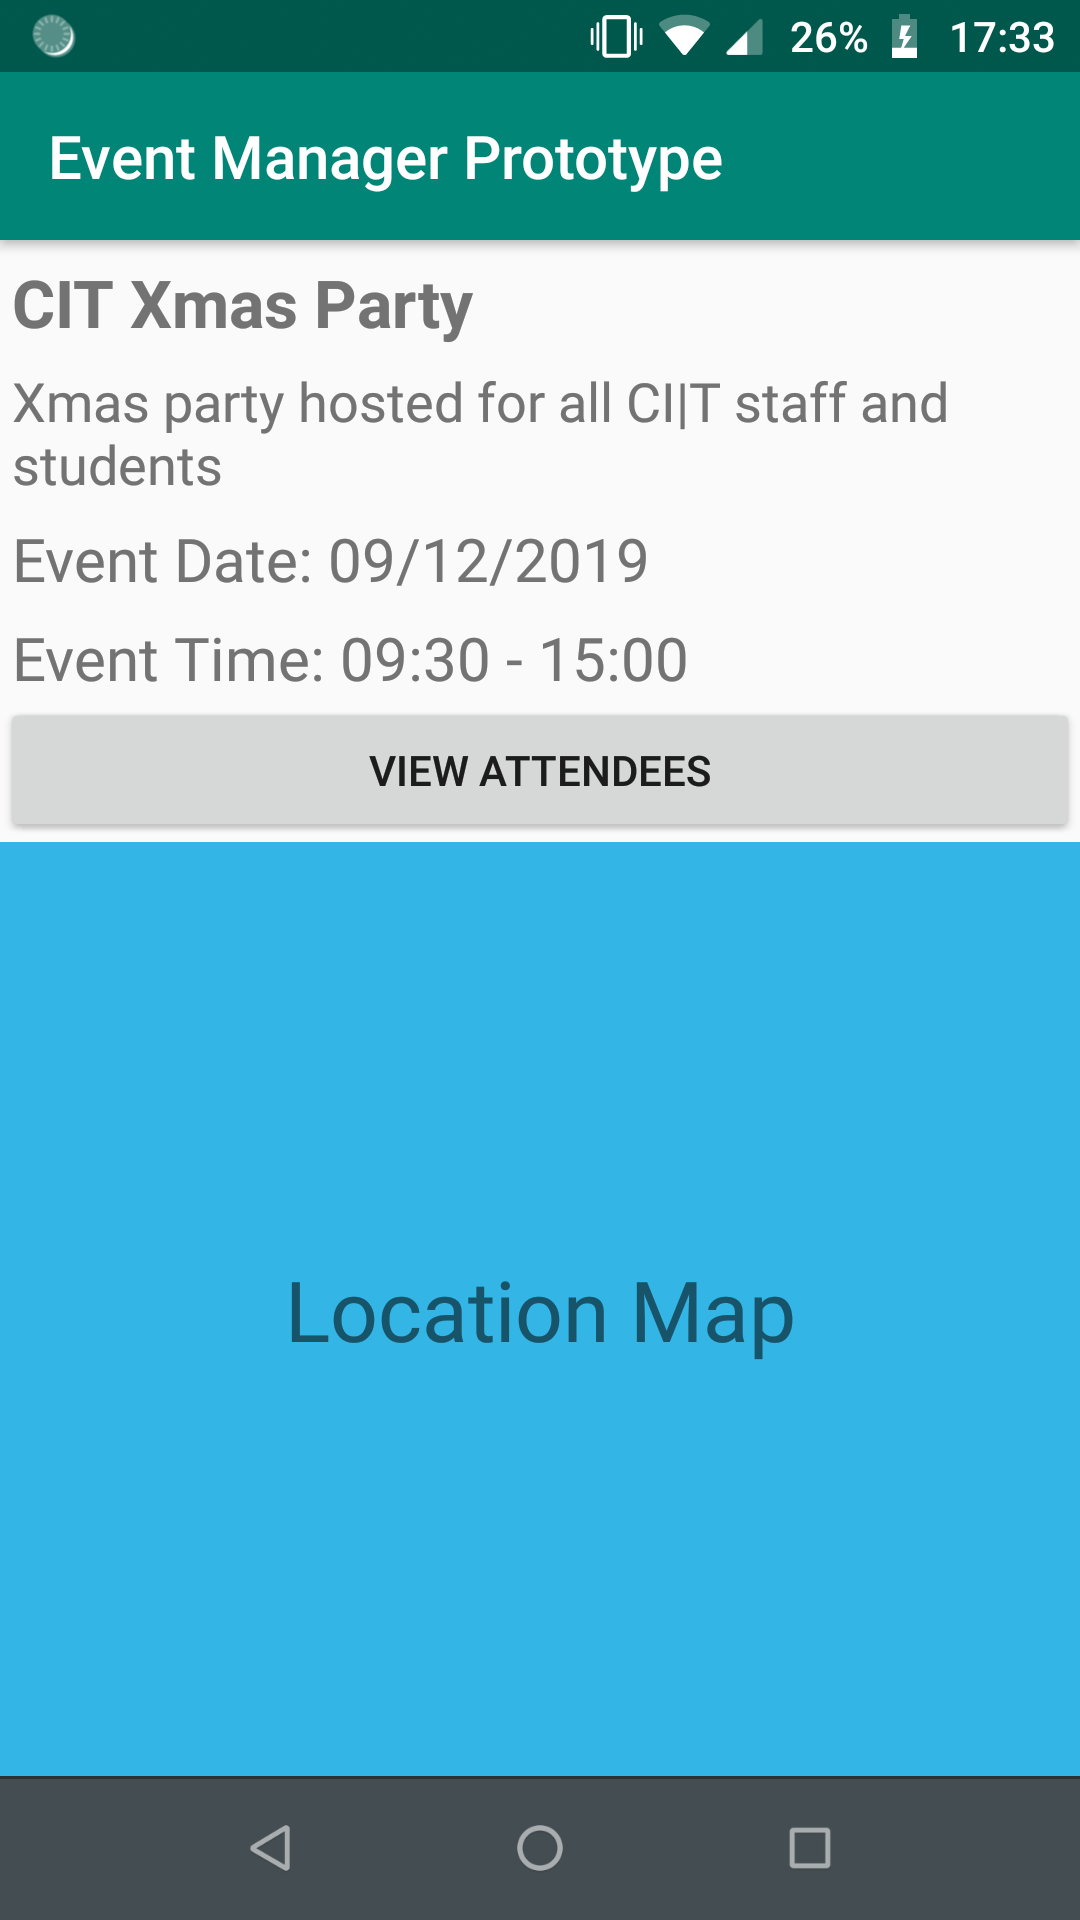
\includegraphics[width=0.7\textwidth]{EventDetail.png}
  \caption[Mobile App Prototype Event Details]{Mobile App Prototype Event Details}
  \label{fig:EventDetail}
\end{figure}

When the user clicks on an event from the events list they will then be provided with further details on that specific event as shown in Figure \ref{fig:EventDetail}. This allows the user to learn about the event in further detail such as viewing other attendees and seeing the event location on a map.

\clearpage
\begin{figure}[ht]
  \centering
      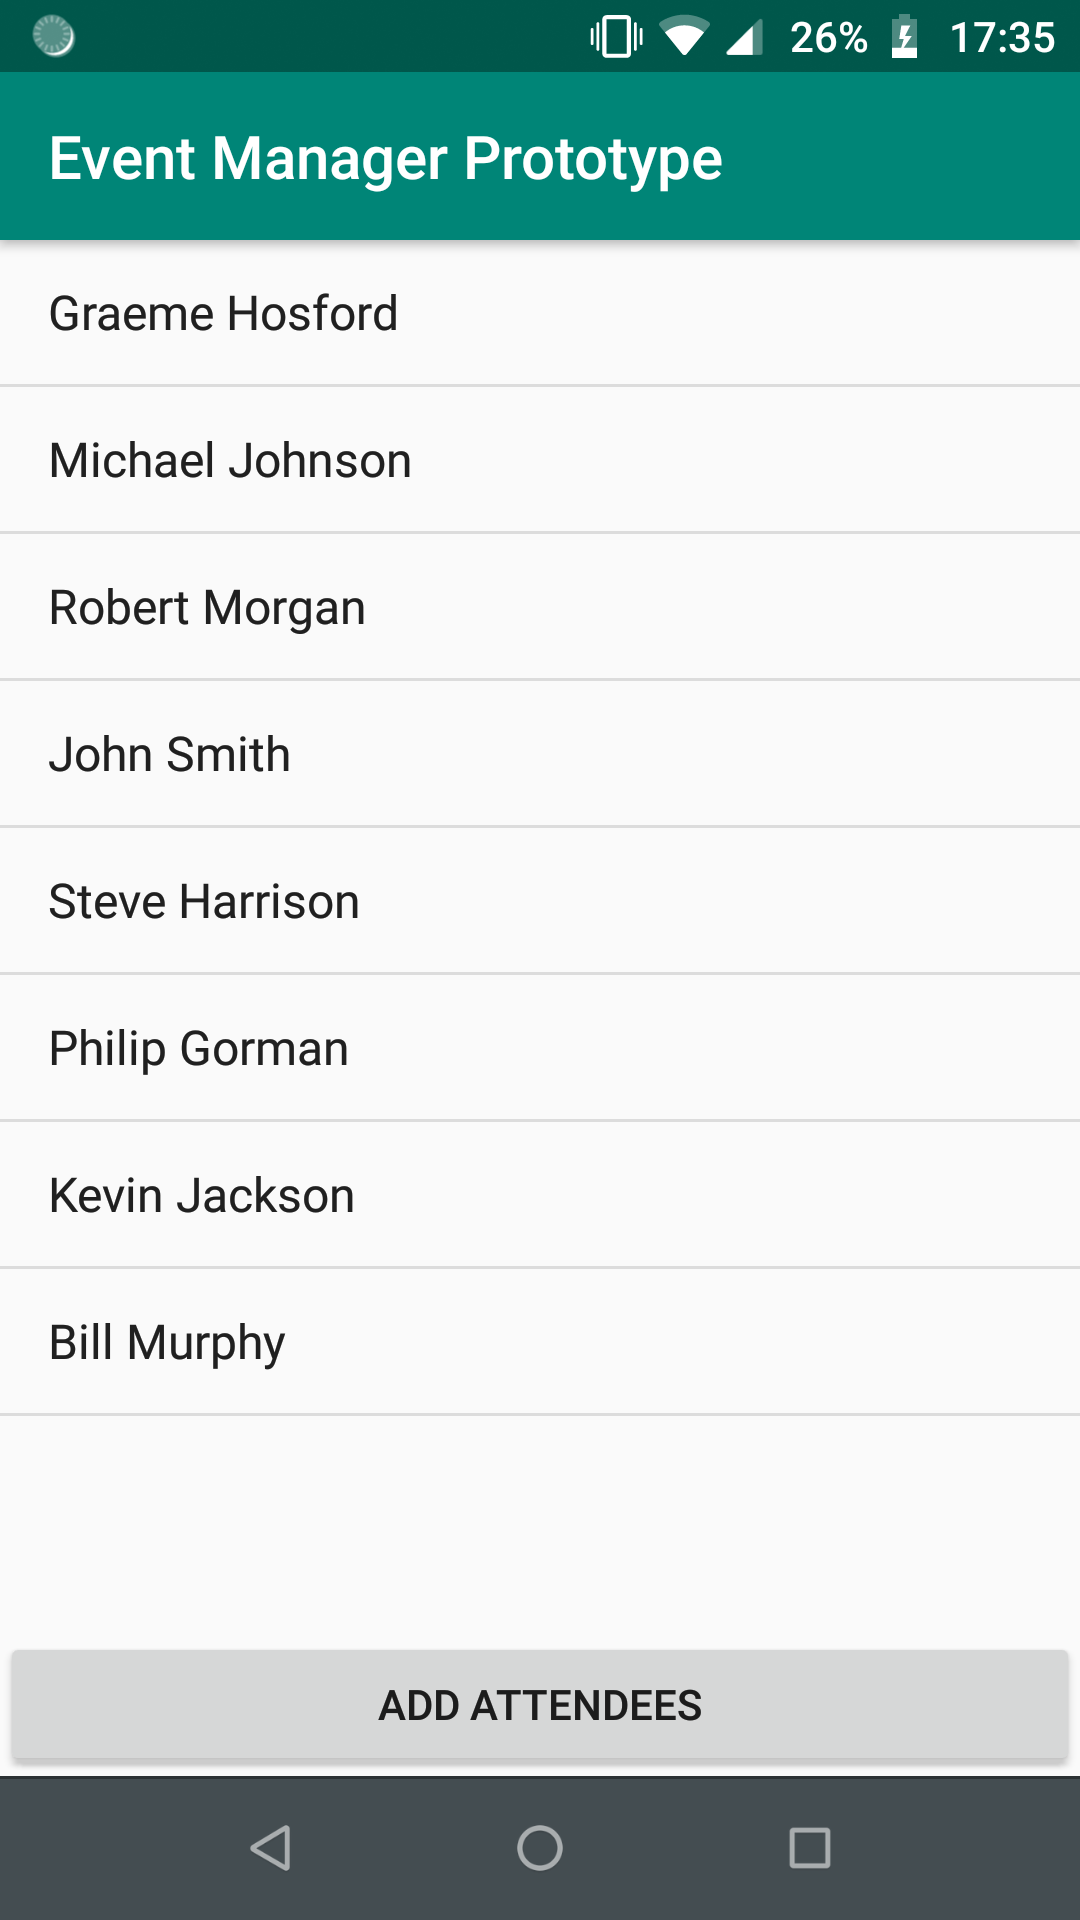
\includegraphics[width=0.7\textwidth]{Attendees.png}
  \caption[Mobile App Prototype Attendees List]{Mobile App Prototype Attendees List}
  \label{fig:AttendeesList}
\end{figure}

The list of attendees for an event can be viewed as shown in Figure \ref{fig:AttendeesList}.

Also provided on this attendees screen is an option to invite more users, this will be an admin-only option and for other users will not be shown.

\clearpage
\begin{figure}[ht]
  \centering
      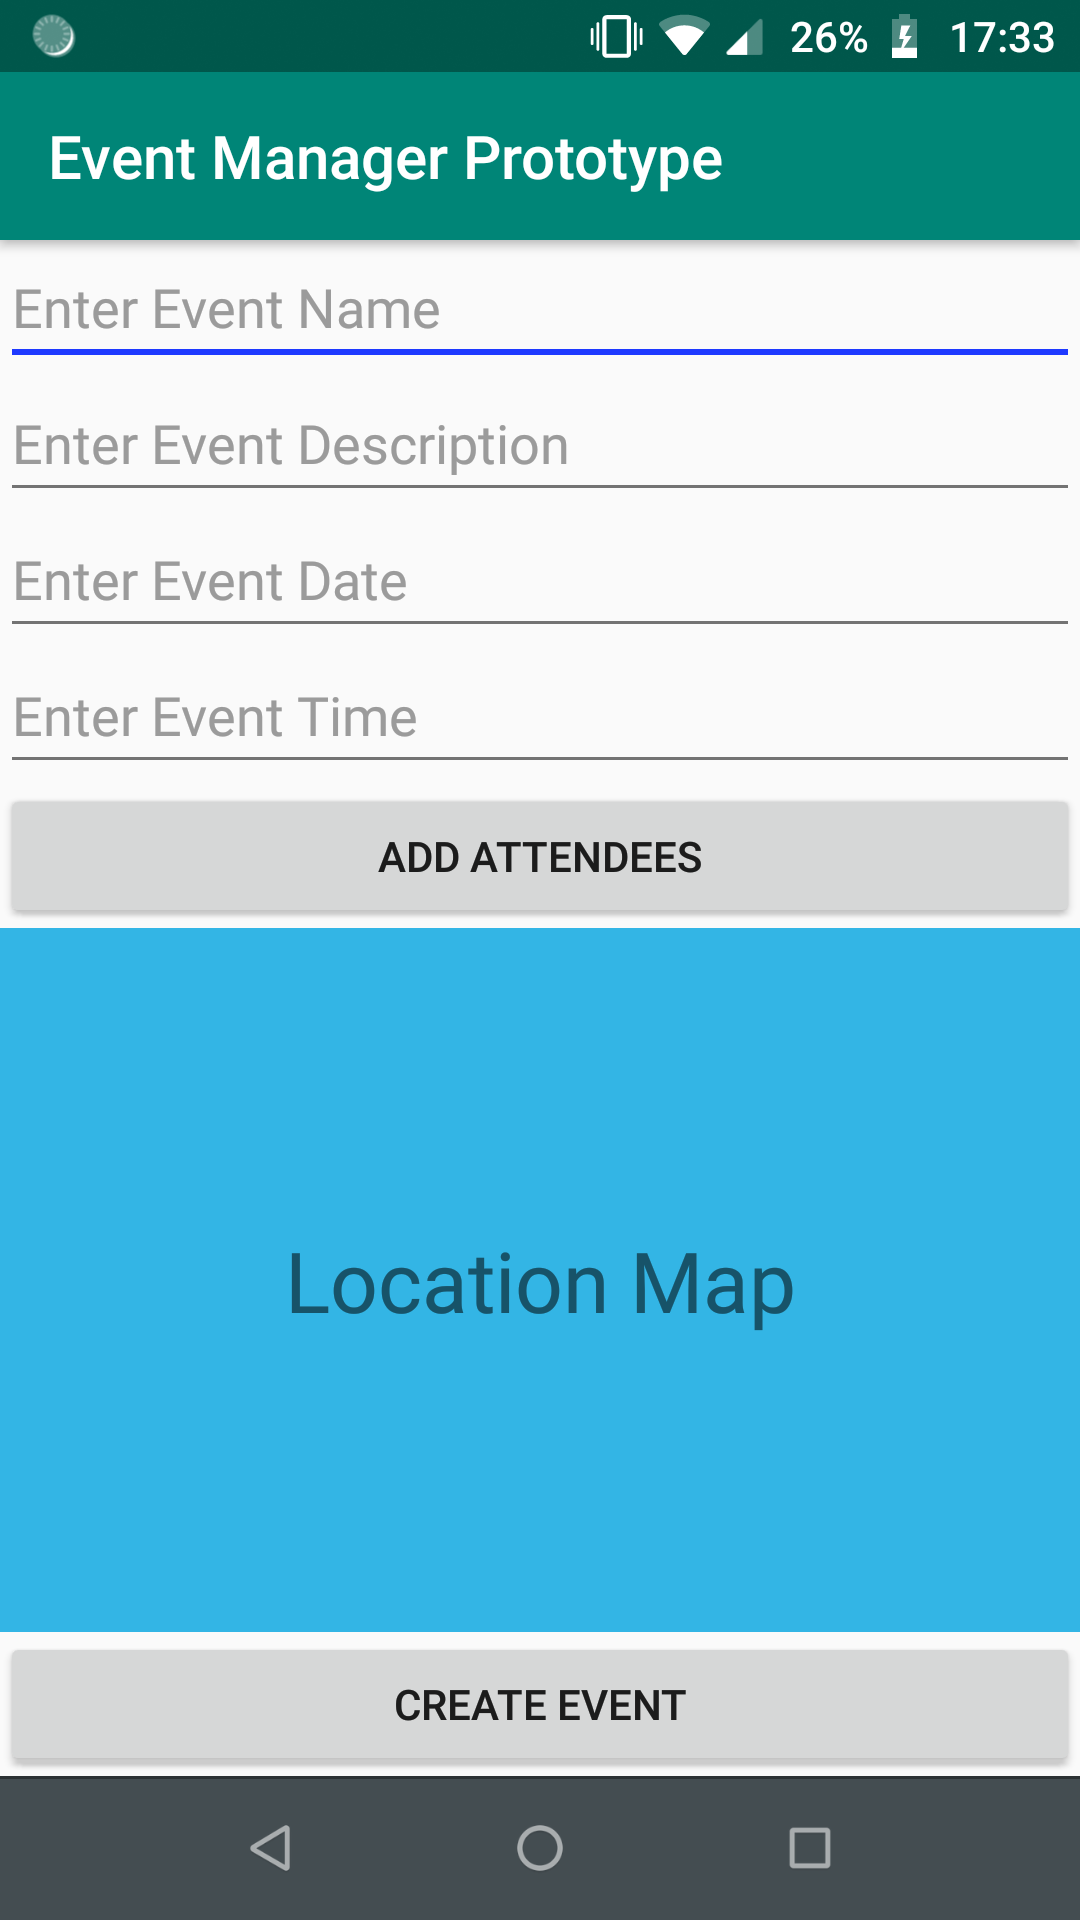
\includegraphics[width=0.7\textwidth]{CreateEvent.png}
  \caption[Mobile App Prototype Create Event Screen]{Mobile App Prototype Create Event Screen}
  \label{fig:CreateEvent}
\end{figure}

When creating an event the screen shown in Figure \ref{fig:CreateEvent} will be presented. This allows the admin to enter the event information which, in turn, will be shown to attendees as in Figure \ref{fig:EventDetail}. The option to add attendees will lead to the same screen as in Figure \ref{fig:AttendeesList}.

\clearpage
\begin{figure}[ht]
  \centering
      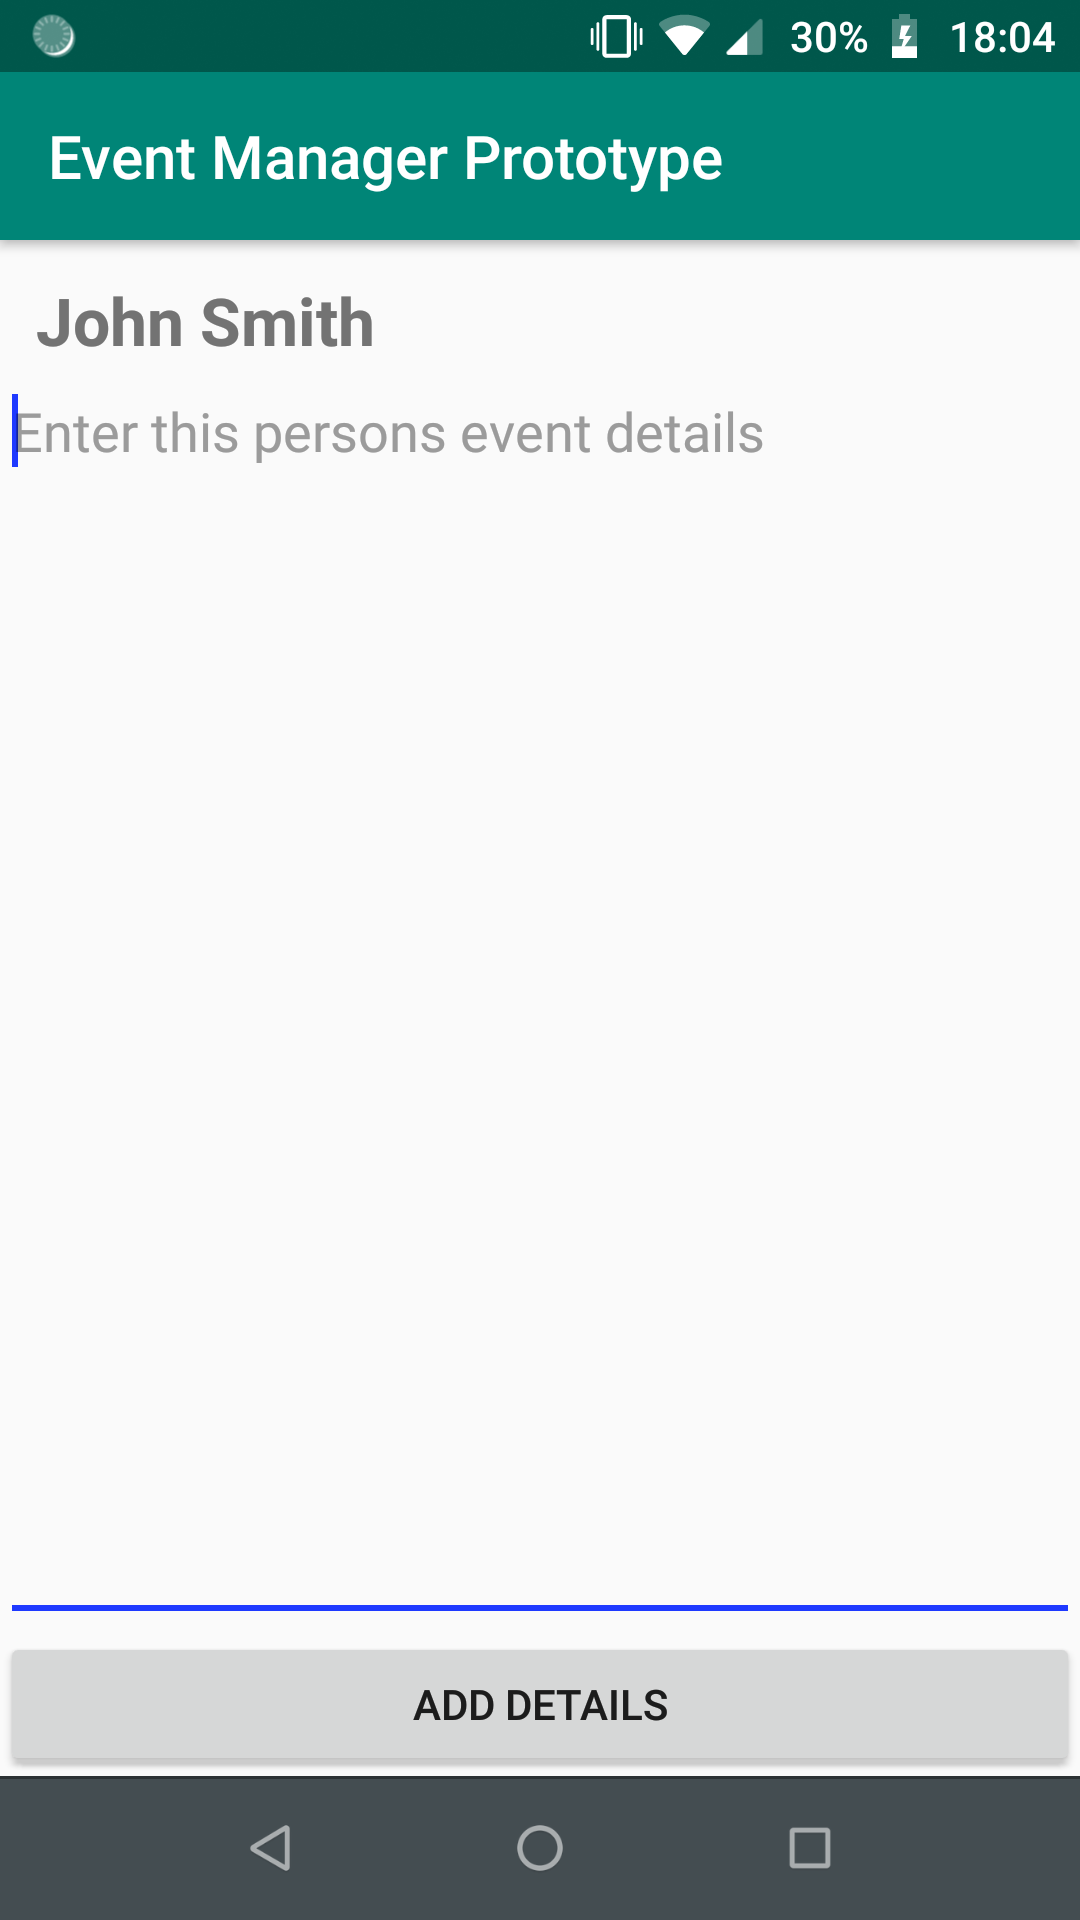
\includegraphics[width=0.7\textwidth]{PersonEventDetails.png}
  \caption[Mobile App Prototype Add Person Event Details Screen]{Mobile App Prototype Add Person Event Details Screen}
  \label{fig:PersonEventDetails}
\end{figure}

When on the attendees list screen as shown in Figure \ref{fig:AttendeesList} an admin may choose to add event specific details to that attendee as shown in Figure \ref{fig:PersonEventDetails}. As there are far too many variable options that an event organiser could add it is deemed easiest to allow a free input through a textbox as shown here rather than trying to create a UI which covers all of the many possibilities.

\clearpage
\begin{figure}[ht]
  \centering
      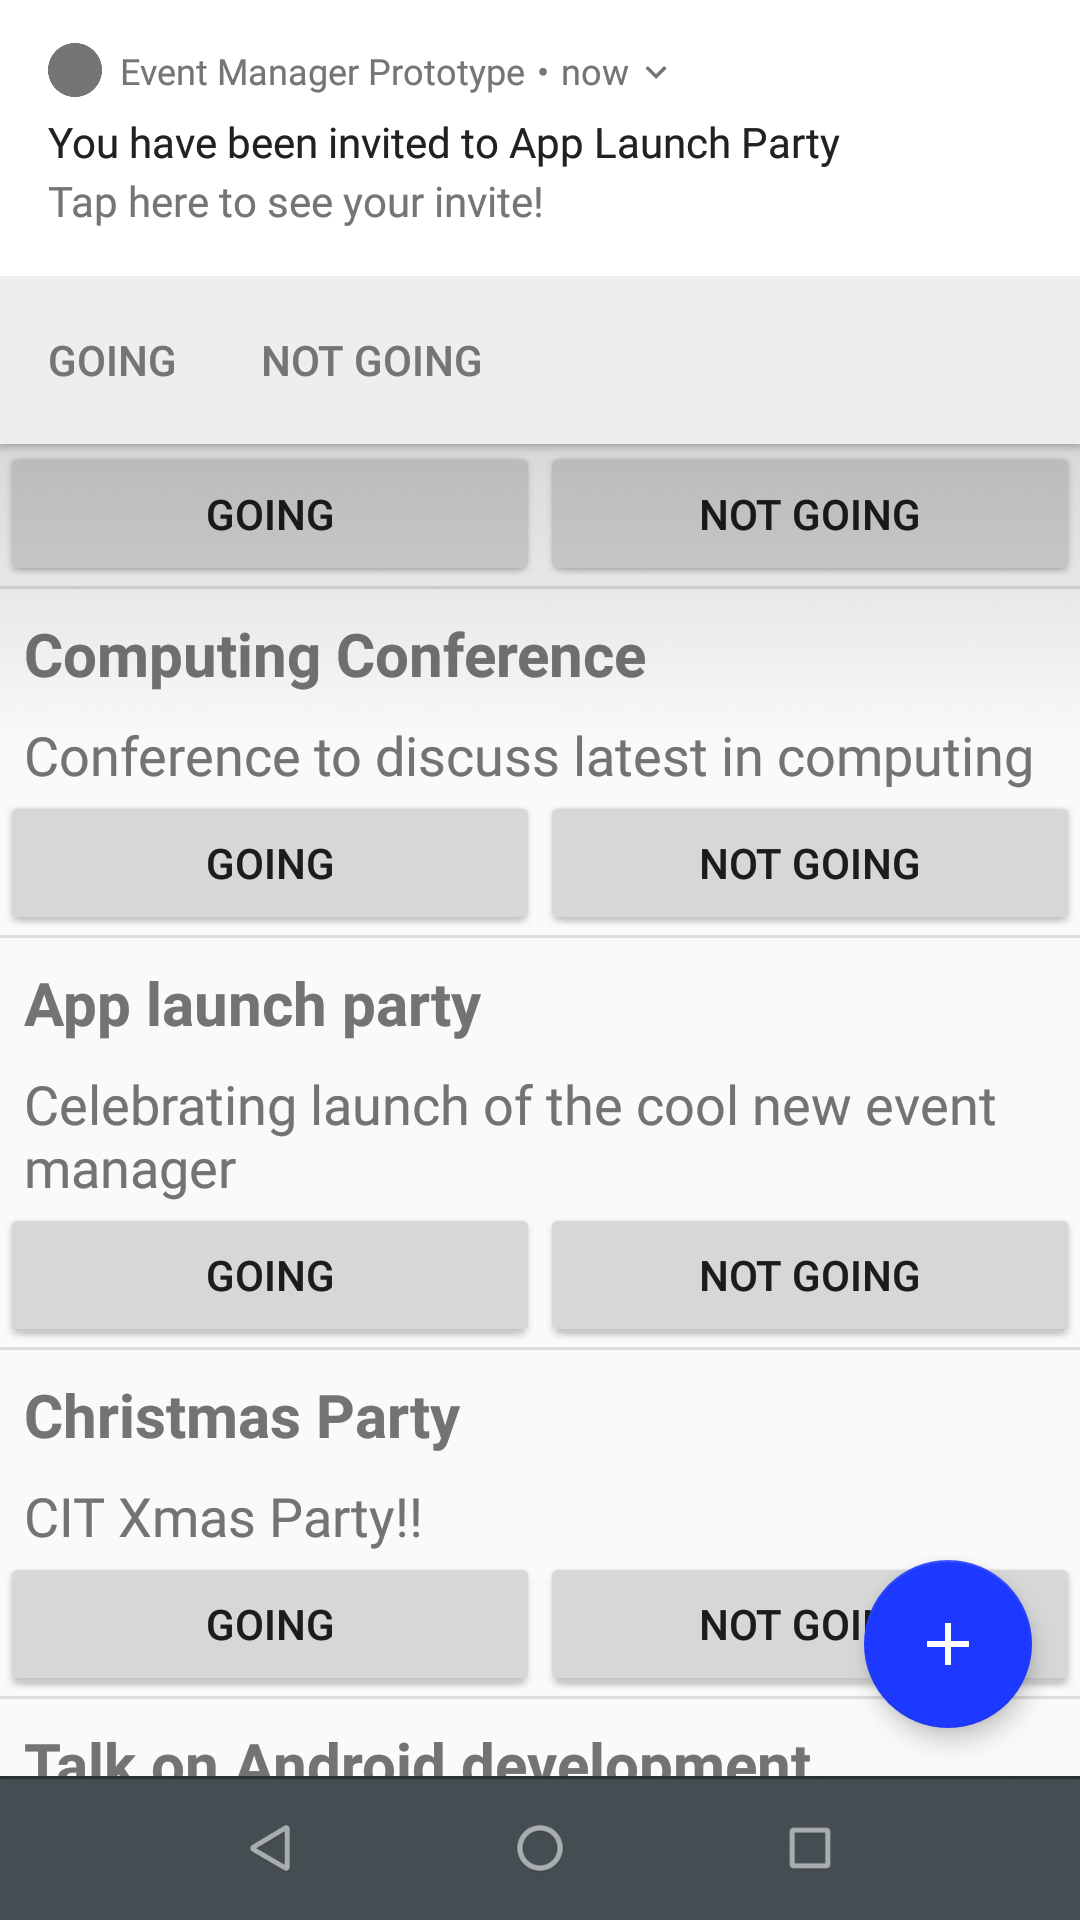
\includegraphics[width=0.7\textwidth]{EventNotification.png}
  \caption[Mobile App Prototype Event Notification Example]{Mobile App Prototype Event Notification Example}
  \label{fig:EventNotification}
\end{figure}

An example of the notifications sent by Firebase when invited to an event is shown in Figure \ref{fig:EventNotification}. A similar notification will be sent when an event thee user has responded to as 'Going' is sent shortly before the event starts as a reminder.

Tapping on the main body of this notification will take the user to view the event details as outlined in Figure \ref{fig:EventDetail}. Also included are shortcut actions to quickly respond to an invite.

\clearpage
\begin{figure}[ht]
  \centering
      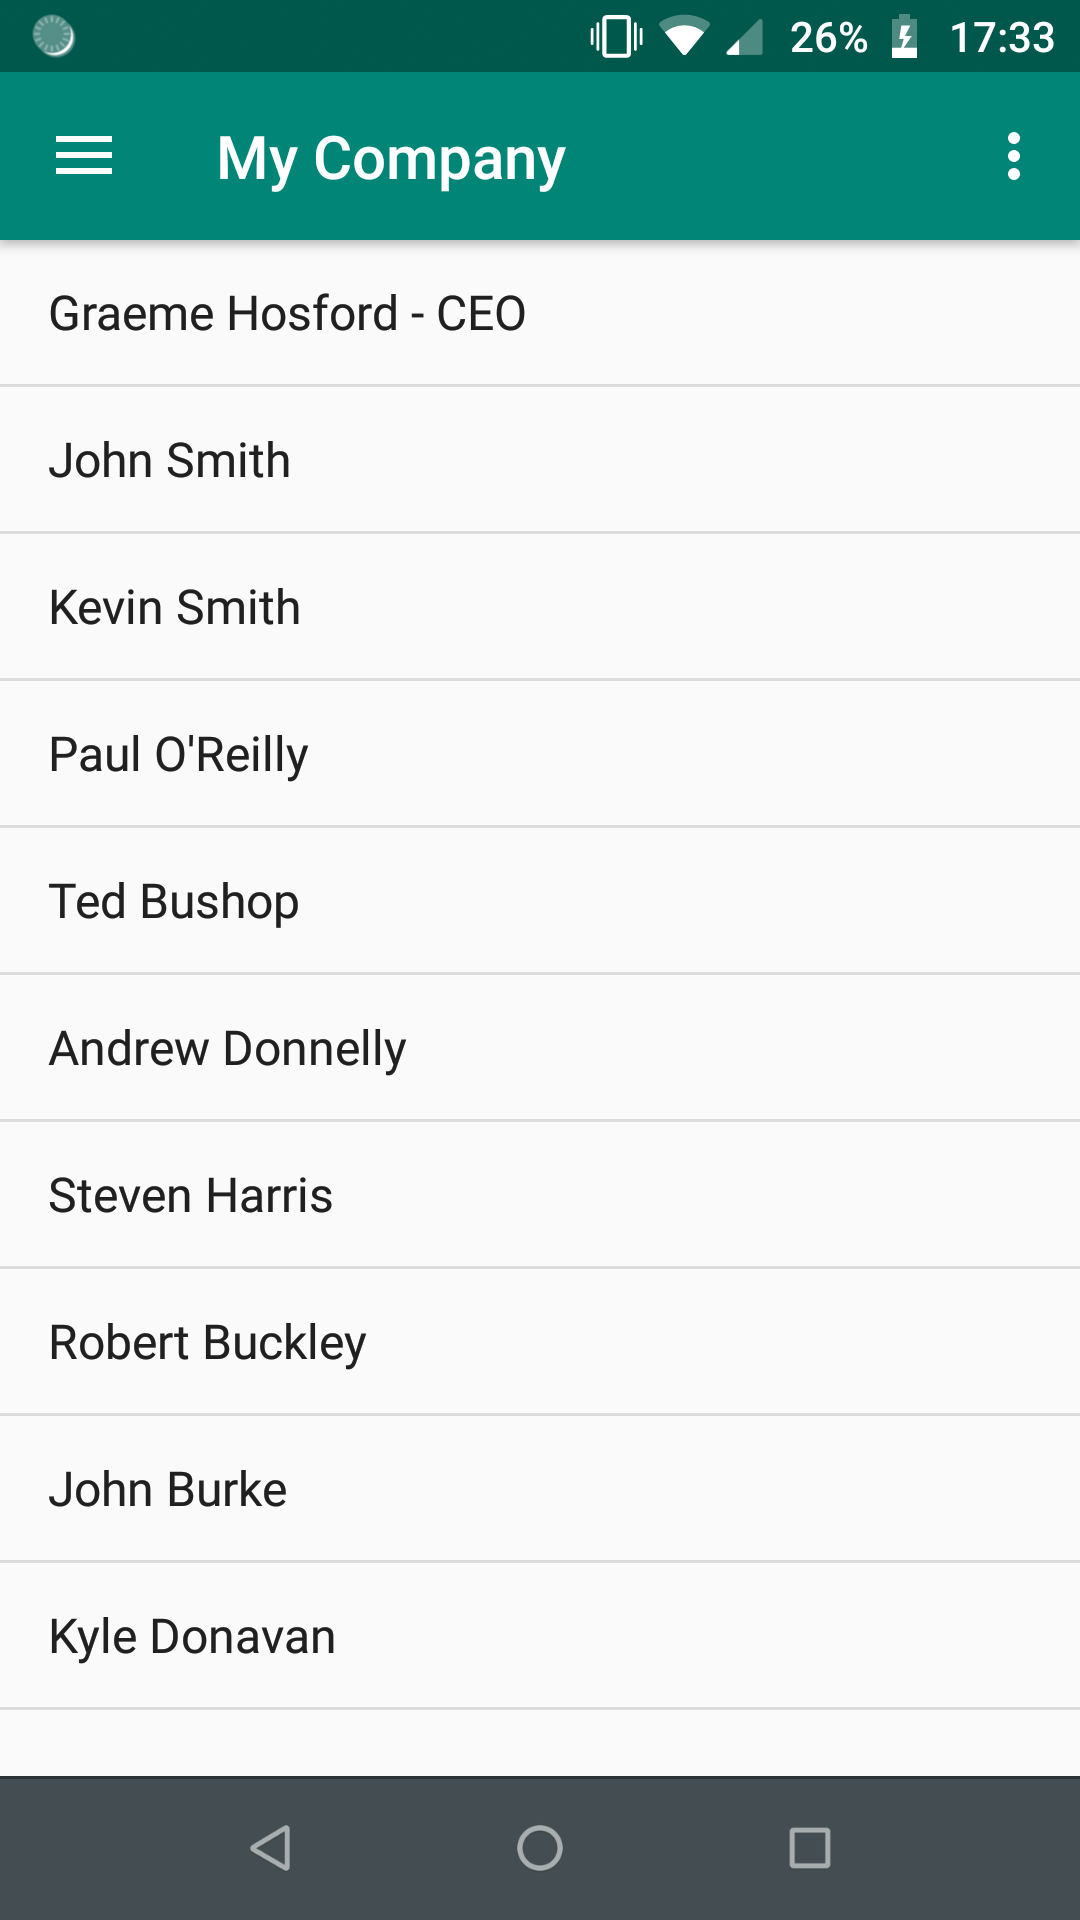
\includegraphics[width=0.7\textwidth]{CompanyMembers.png}
  \caption[Mobile App Prototype Company Details Screen]{Mobile App Prototype Create Company Details Screen}
  \label{fig:CompanyDetails}
\end{figure}

As shown in Figure \ref{fig:CompanyDetails} the user can view the list of members of their own company.

\clearpage
\begin{figure}[ht]
  \centering
      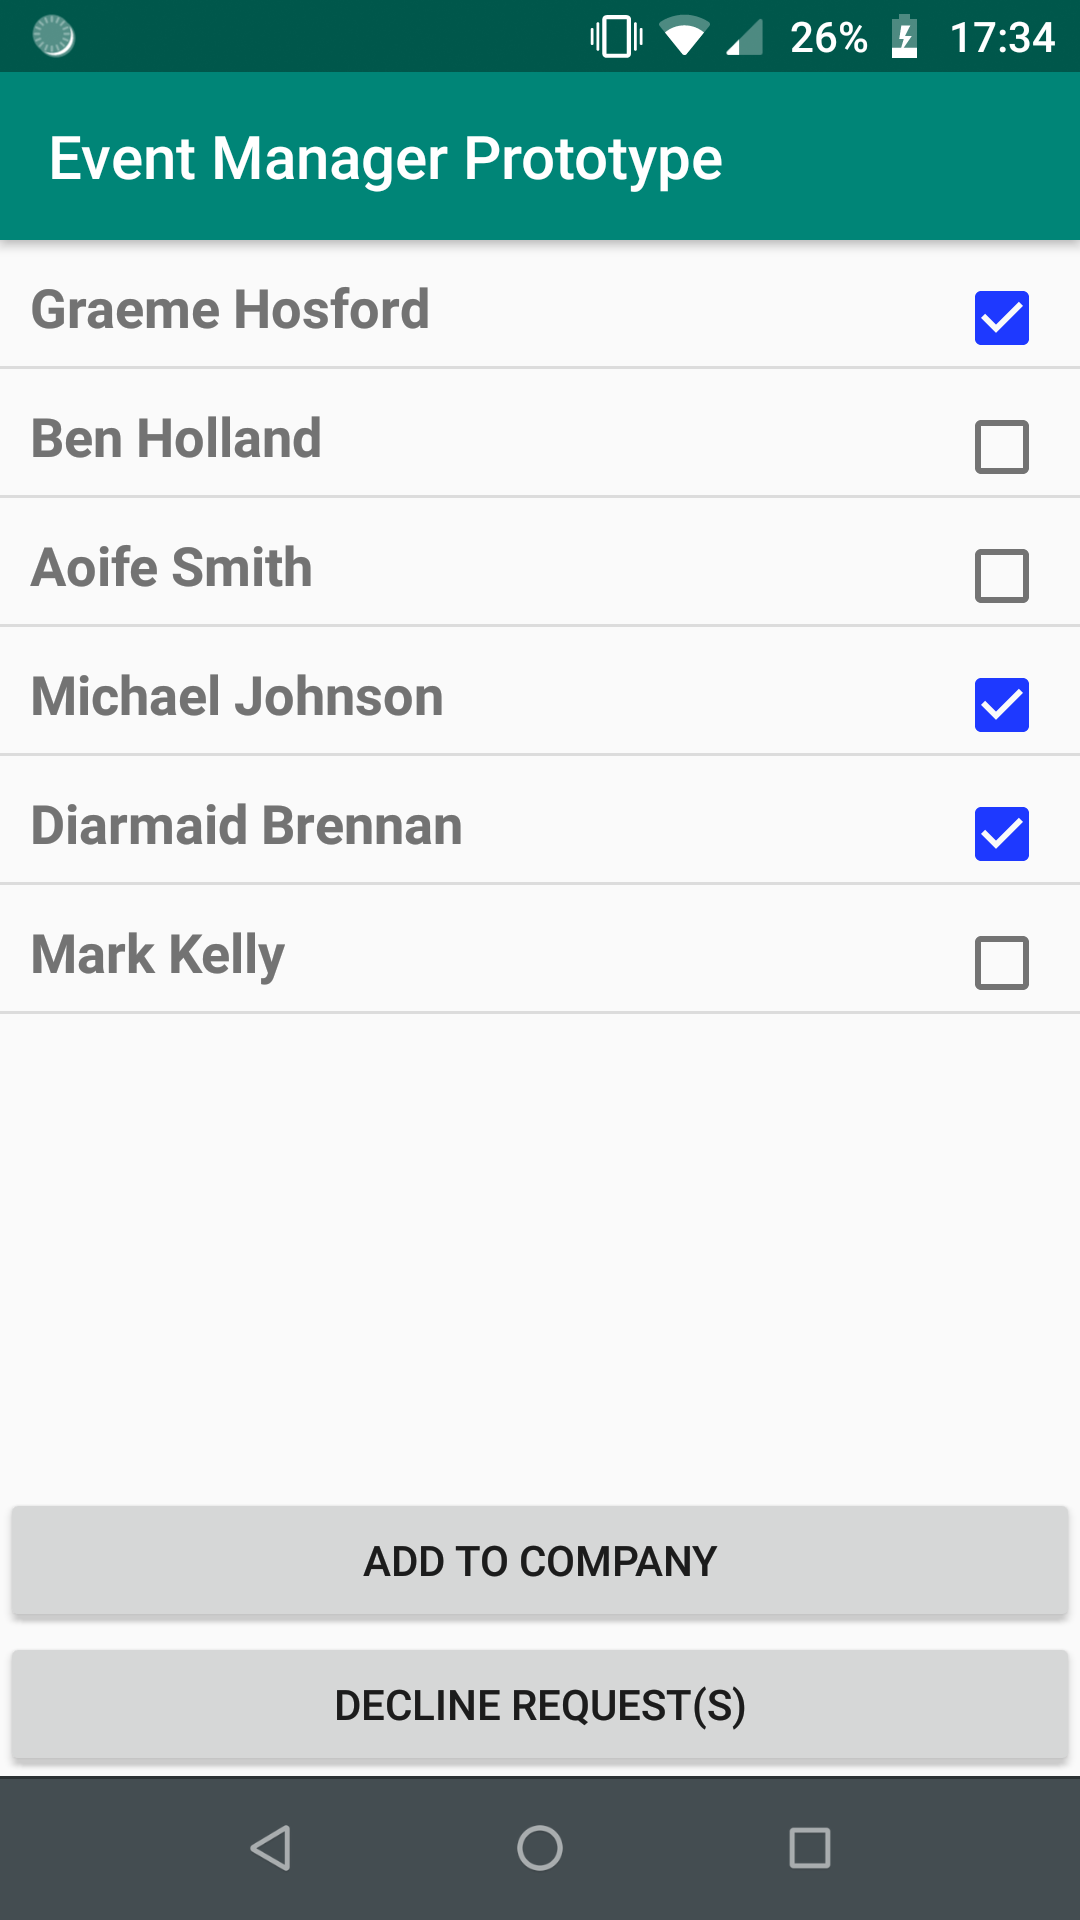
\includegraphics[width=0.7\textwidth]{MemberRequests.png}
  \caption[Mobile App Prototype Company Member Requests Screen]{Mobile App Prototype Company Member Requests Screen}
  \label{fig:MemberRequests}
\end{figure}

In Figure \ref{fig:MemberRequests} is the admin-only feature of approving or denying member requests for the company. Any users added from this list is able to view the company's events and members, and any user whose request is declined simply has their request removed from this list.

\clearpage
\begin{figure}[ht]
  \centering
      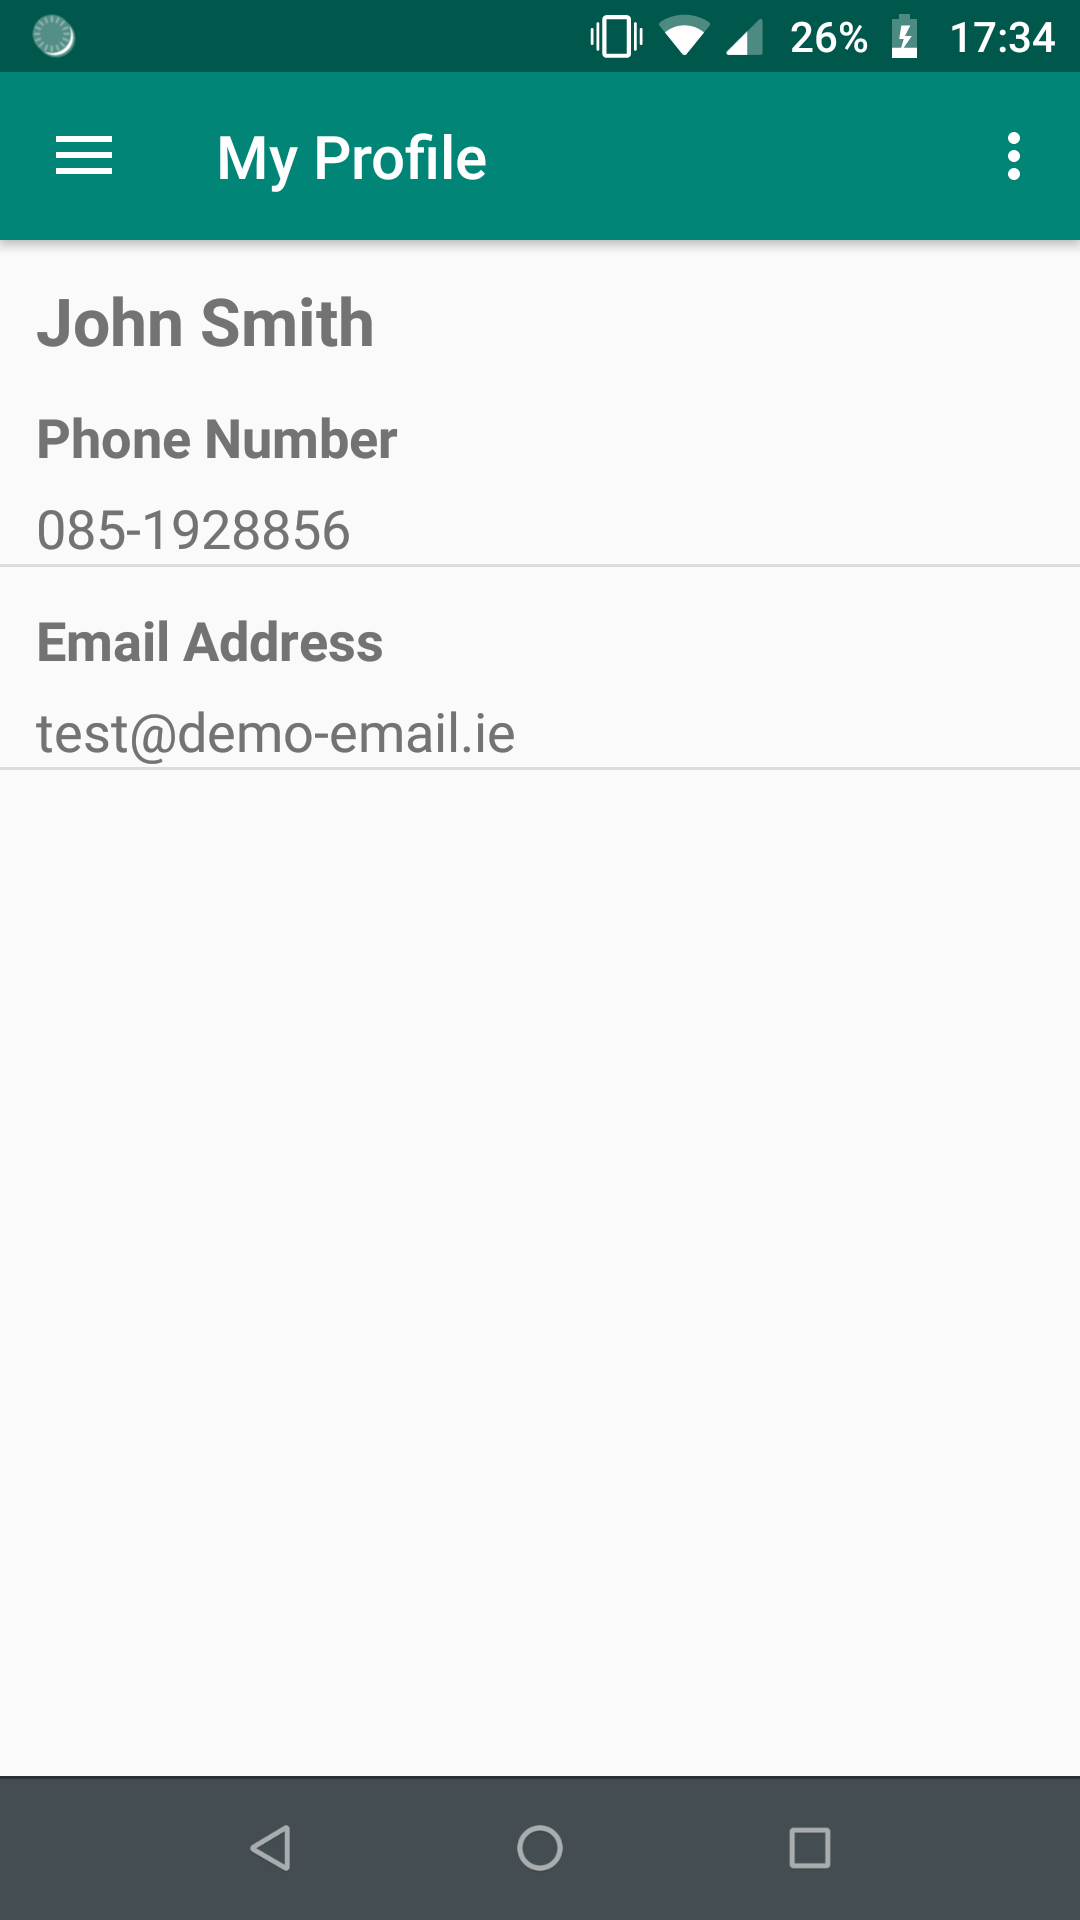
\includegraphics[width=0.7\textwidth]{Profile.png}
  \caption[Mobile App Prototype User Profile Screen]{Mobile App Prototype User Profile Screen}
  \label{fig:UserProfile}
\end{figure}

A user profile is shown in Figure \ref{fig:UserProfile}. A user can view their own profile through choosing the option from the main navigation menu or selecting their own name from the list of company members. The profiles of other user can also be accessed through the member list. 

When a user is on their own profile they also have the option of editing it to change and update the information shown there.

\clearpage % Forcing on to a new page to stop overlap between mobile app and ruby prototypes - Figures are very awkward :/
\subsection{Ruby Server Prototype}

In this section is just the prototype JSON responses for when a new company is created. Unfortunately it was not possible to prototype the notification scheduling here, as again this is mainly Firebase related. Also it was not possible to demonstrate a delayed action. Some prototype output for this however can be seen in Figure \ref{fig:EventNotification}.

\begin{figure}[ht]
  \centering
      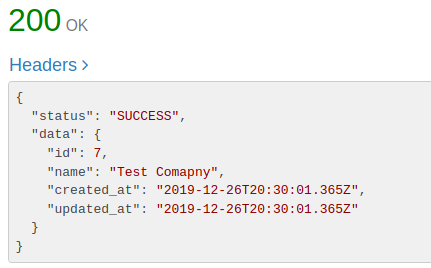
\includegraphics[width=0.7\textwidth]{CompanyPOSTExample.PNG}
  \caption[Ruby Server Prototype Create Company Response]{Ruby Server Prototype Create Company Response}
  \label{fig:CompanyPOST}
\end{figure}

Shown in Figure \ref{fig:CompanyPOST} is the response generated when a new company has been created by the Ruby on Rails server. The key part of this response is the "id" field. As mentioned before the default implementation of Ruby on Rails will automatically generate a simple human readable ID through its database implementation. This ID is then forever associated with the created company and can be entered by users to request to join a company as outlined in Figure \ref{fig:CreateJoinCompany}.